\chapter{Flashing the FPGAs and CPLDs in the MEGA65}
\label{cha:fpgacpldflashing}

The MEGA65 is an open-source and open-hardware computer. This means you are free,
not only to write programs that run on the MEGA65 as a finished computer, but also to
use the re-programmable chips in the MEGA65 to turn it into all sorts of other things.

If you just want to install an upgrade core for the MEGA65, or a core that lets you use
your MEGA65 as another type of computer, you probably want to look in
\bookvref{cha:cores} instead.

This chapter is more intended for people who want to help develop cores for the MEGA65. This chapter may also be of interest to Nexys4 board owners that are interested booting their devices from the on-board QSPI flash memory chip (rather than a bitstream file on the SD card). This will require flashing an .mcs file onto their board's QSPI chip, so as to provide an initial bistream in the 'Slot 0' position.

These re-programmable chips are called Field Programmable Gate Arrays (FPGAs) or
Complex Programmable Logic Devices (CPLDs), and can implement a wide variety of circuits.
They are normally programmed using a language like VHDL or Verilog.  These
are languages that are not commonly encountered by most people.  They are also quite
different in some ways to ``normal'' programming languages, and it can take a while to
understand how they work. But with some effort and perseverance, exciting things can be created with them.

\section{Suggested PC specifications}

Be prepared to install many gigabytes of software on a Linux or Windows PC, before you will
be able to write programs for the FPGAs and CPLDs in the MEGA65.  Also,
"compiling" complex
designs can take up to several hours, depending on the speed and memory
capacity of your computer.
We recommend a computer with at least 12GB RAM (preferably 16GB) if you want to write
programs for FPGAs and CPLDs. On the other hand, if all you want to do is load programs onto
your MEGA65's FPGAs and CPLDs that other people have written, then most
computers running a recent
version of Windows or Linux should be able to cope.

\begin{itemize}
  \item \underline{OS}: Linux or Windows
  \item \underline{CPU Speed}: As fast as you can get your hands on!
  \item \underline{Number of cores}: Ideally, 8 or more, as the free license of Vivado can make use of a max of 8 cores.
  \item \underline{Hard disk space}: Have about 70GB or more. The exact amount used depends on how many components within Vivado you install (bear in mind that the full install file is about 50GB in itself)
  \item \underline{Memory}: minimum of 12GB (ideally, have more, to play it safe)
\end{itemize}

\section{Warning}

Before we go any further, we do have to provide a warning about reprogramming the FPGAs and
CPLDs in the MEGA65.
Re-programming the MEGA65 FPGA can potentially cause
damage, or leave your MEGA65 in an unresponsive state from which it is very difficult to
recover, i.e., ``bricked''.  Therefore if you choose to open your MEGA65 and reprogram
any of the FPGAs it contains, it is no longer possible to guarantee its correct operation.
Therefore, we cannot reasonably honour the warranty of the
device as a computer.
You have been warned!

\section{Installing Vivado}
\label{sec:installvivado}

Installation of Vivado is required to flash the QSPI flash memory within your MEGA65 target device, whether it be a MEGA65 R2/R3/R3A/R4, Nexys4/Nexys4DDR/NexysA7, MEGAphone or other.

Vivado is also the tool used to perform compilation (synthesis, as it is preferably called) of FPGA bitstreams.

To get started, connect to \url{https://www.xilinx.com/support/download.html}

\begin{minipage}{\linewidth}
  Select 2020.2 version
  \\
  \begin{center}
    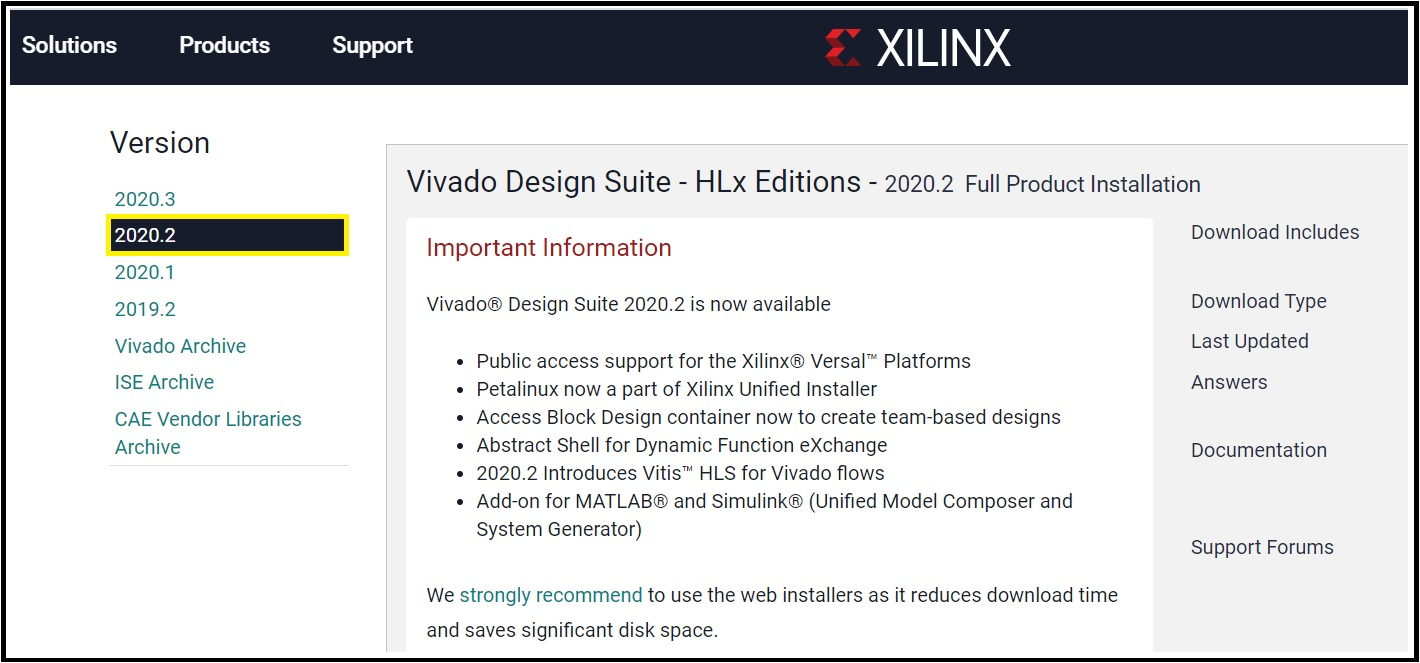
\includegraphics[width=\linewidth]{images/VivadoInstimg002.jpg}
  \end{center}
  NOTE : Some users still have success with using older versions, as the main aim here is to install a version that supports the FPGA of your target hardware. \\
  \\
  I.e., the Artix7 100T (for Nexys and R2) or 200T (R3/R3A/R4).
\end{minipage}

\begin{minipage}{\linewidth}
  Click on Xilinx Unified Installer 2020.2: Windows Self Extracting Web Installer EXE - 248.44MB
  \\
  \begin{center}
    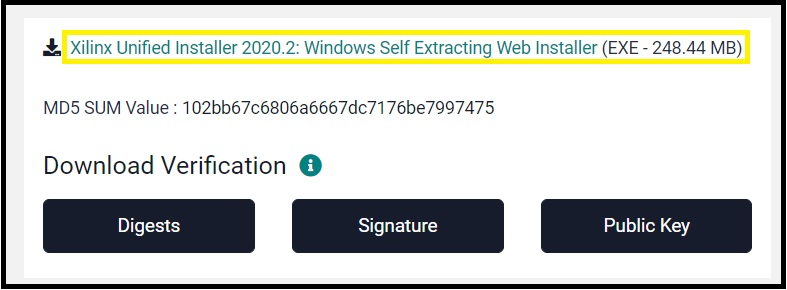
\includegraphics[width=0.8\linewidth]{images/VivadoInstimg003.jpg}
  \end{center}
\end{minipage}

\begin{minipage}{\linewidth}
  You will be asked to create an account in order to sign in and be able to download the installation program. \\
  \\
  Your credentials will also be requested when doing the installation.
  \\
  \begin{center}
    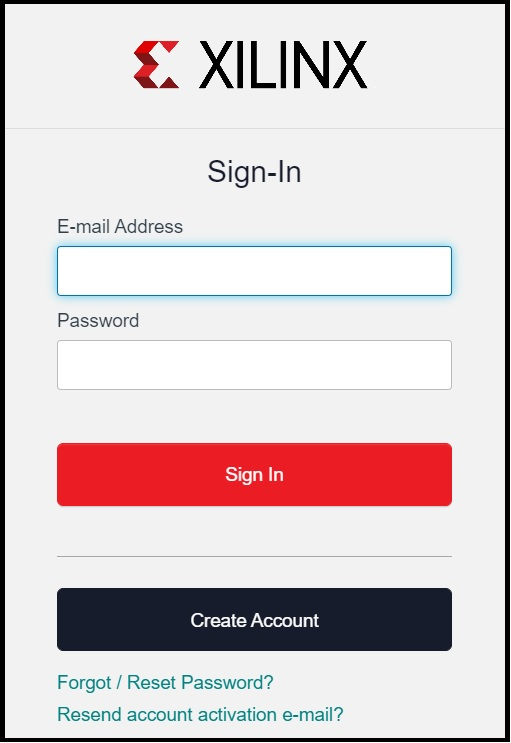
\includegraphics[width=0.3\linewidth]{images/VivadoInstimg004.jpg}
  \end{center}
\end{minipage}

\begin{minipage}{\linewidth}
  After having signed in, you have to provide some personal information and then click on Download
  \\
  \begin{center}
    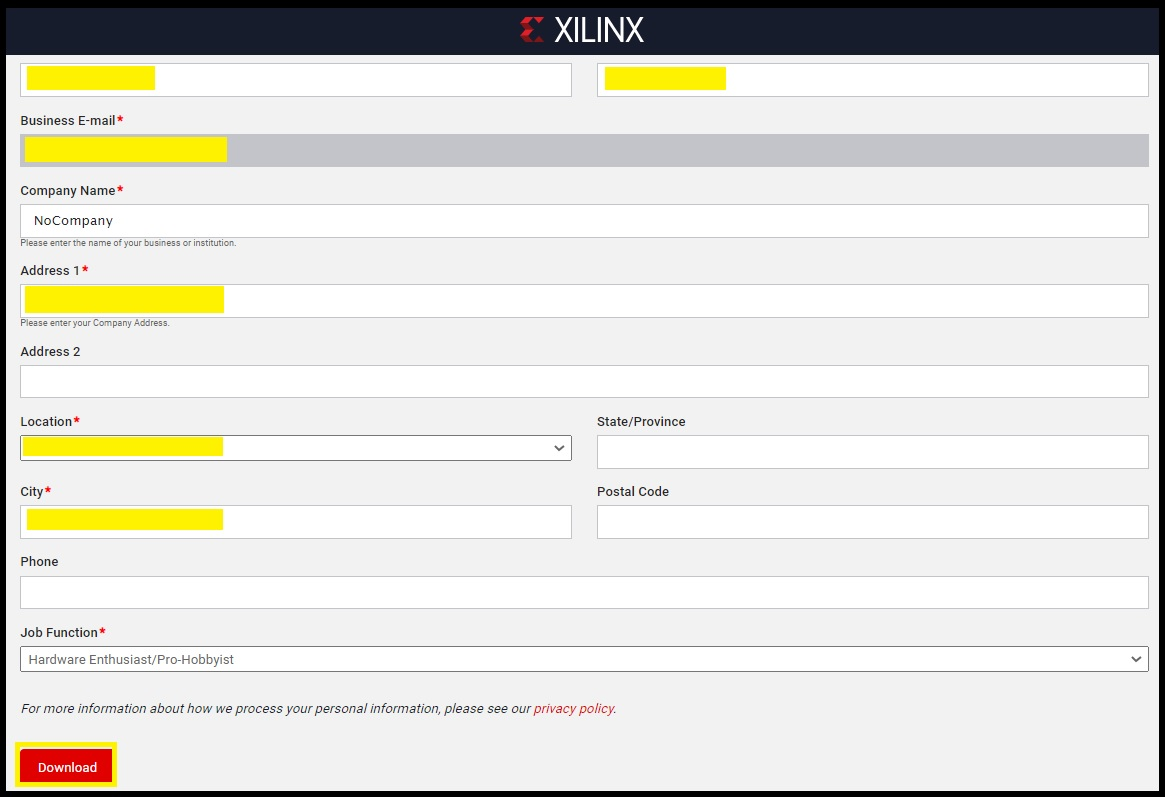
\includegraphics[width=0.8\linewidth]{images/VivadoInstimg005.jpg}
  \end{center}
\end{minipage}

\begin{minipage}{\linewidth}
  Execute the installer as Administrator (Xilinx\_Unified\_2020.2\_1118\_1232\_Win64.exe).
  \\
  \begin{center}
    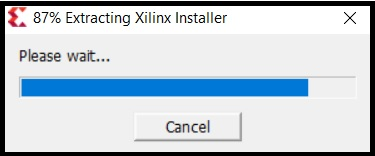
\includegraphics[width=0.5\linewidth]{images/VivadoInstimg006.jpg}
  \end{center}
\end{minipage}

\begin{minipage}{\linewidth}
  Click on Allow Access.
  \\
  \begin{center}
    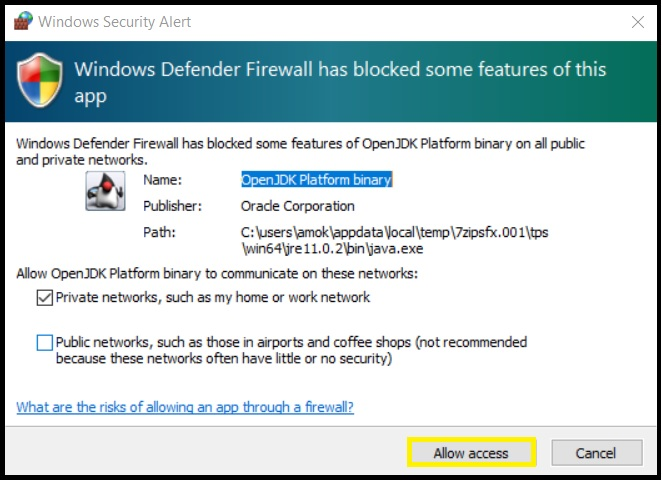
\includegraphics[width=0.5\linewidth]{images/VivadoInstimg007.jpg}
  \end{center}
\end{minipage}

\begin{minipage}{\linewidth}
  Click on Next.
  \\
  \begin{center}
    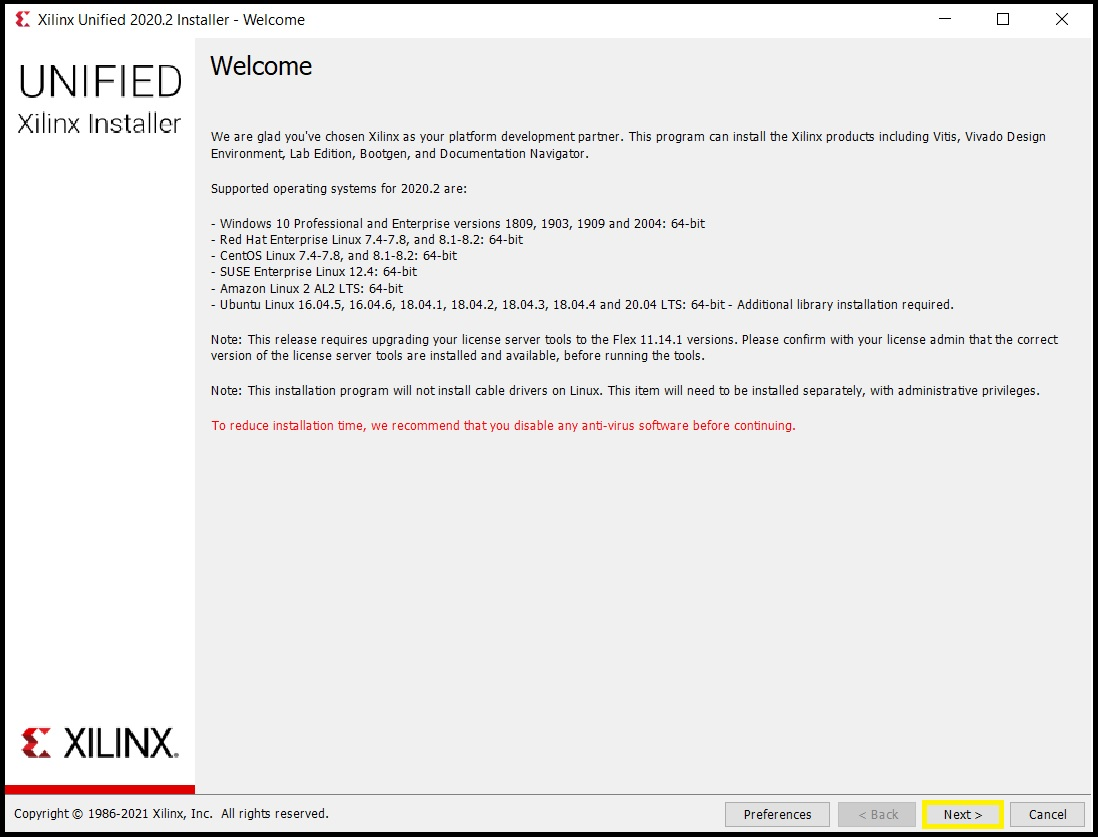
\includegraphics[width=0.7\linewidth]{images/VivadoInstimg008.jpg}
  \end{center}
\end{minipage}

\begin{minipage}{\linewidth}
  Enter your credentials and click on Next.
  \\
  \begin{center}
    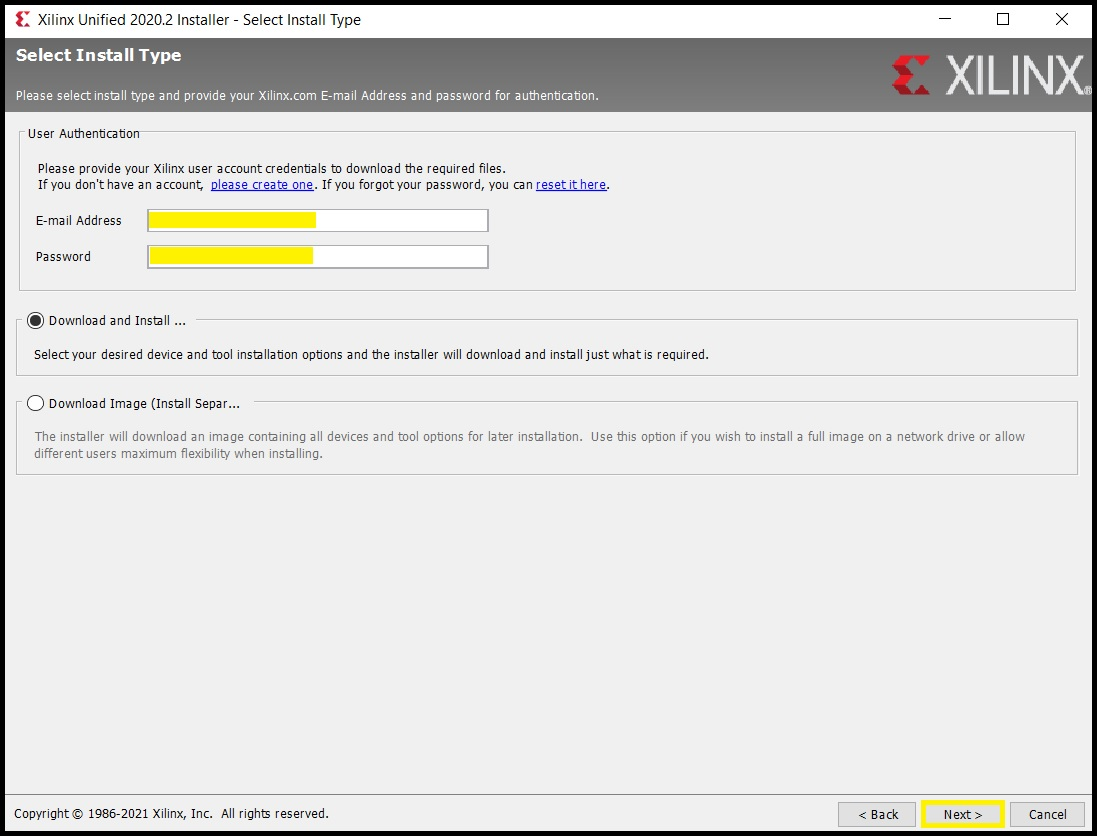
\includegraphics[width=0.7\linewidth]{images/VivadoInstimg009.jpg}
  \end{center}
\end{minipage}

\begin{minipage}{\linewidth}
  Select Vivado and click on Next.
  \\
  \begin{center}
    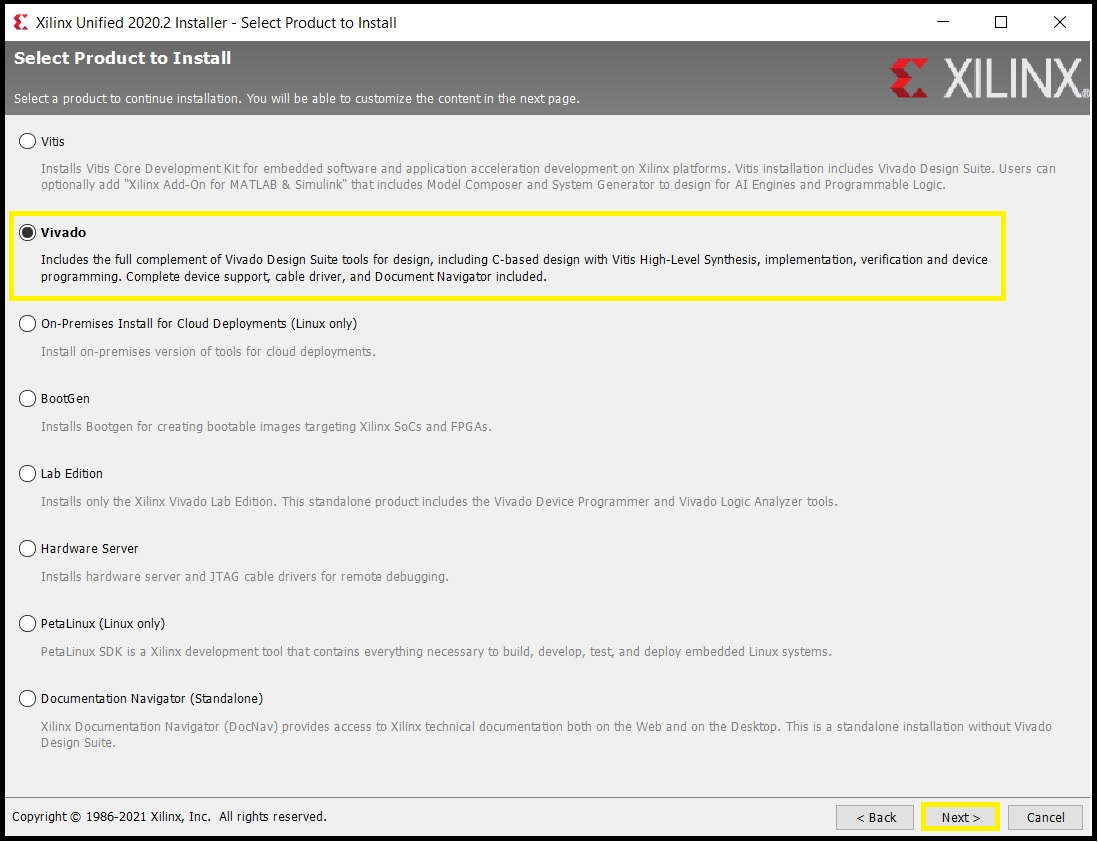
\includegraphics[width=0.7\linewidth]{images/VivadoInstimg010.jpg}
  \end{center}
\end{minipage}

\begin{minipage}{\linewidth}
  Select "Vivado HL WebPACK" and click on "Next"
  \\
  \begin{center}
    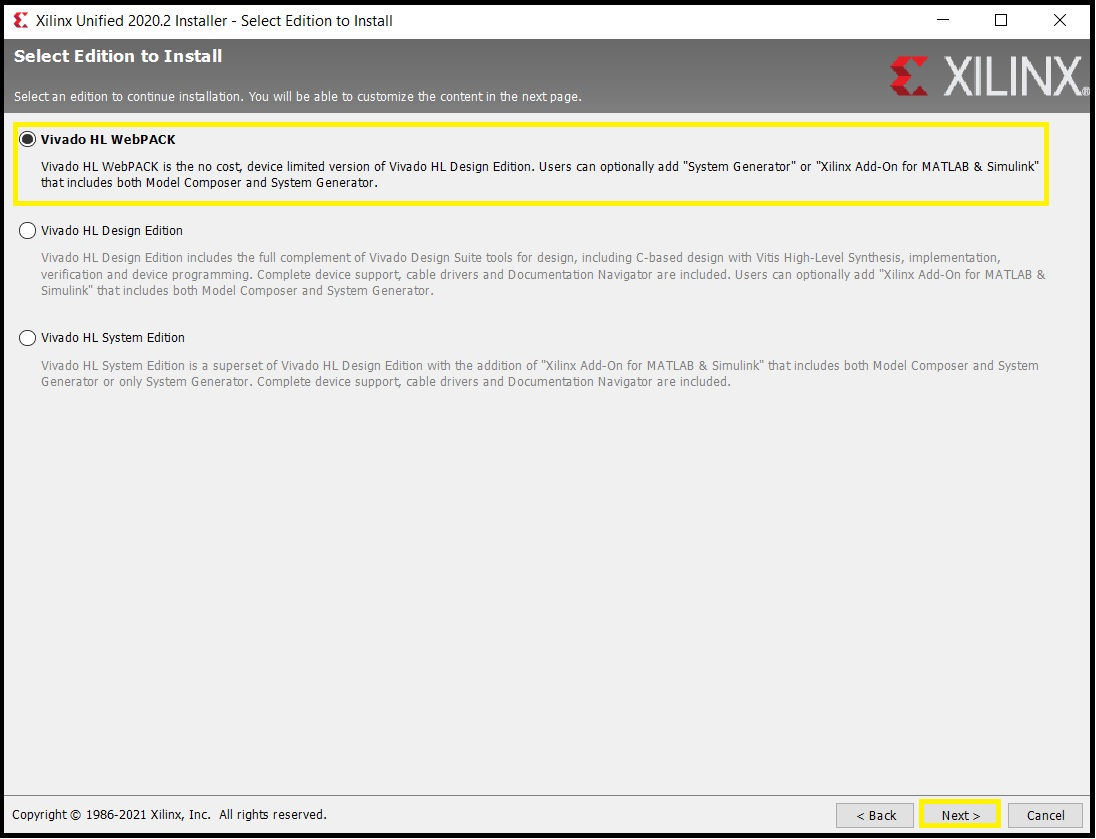
\includegraphics[width=0.7\linewidth]{images/VivadoInstimg011.jpg}
  \end{center}
\end{minipage}

\begin{minipage}{\linewidth}
  We'd suggest selecting only the "\textbf{7 Series}" devices, as our chosen FPGA is within this series, and de-selecting the other series will save you about 6GB in download size. Then click on "Next"
  \\
  \begin{center}
    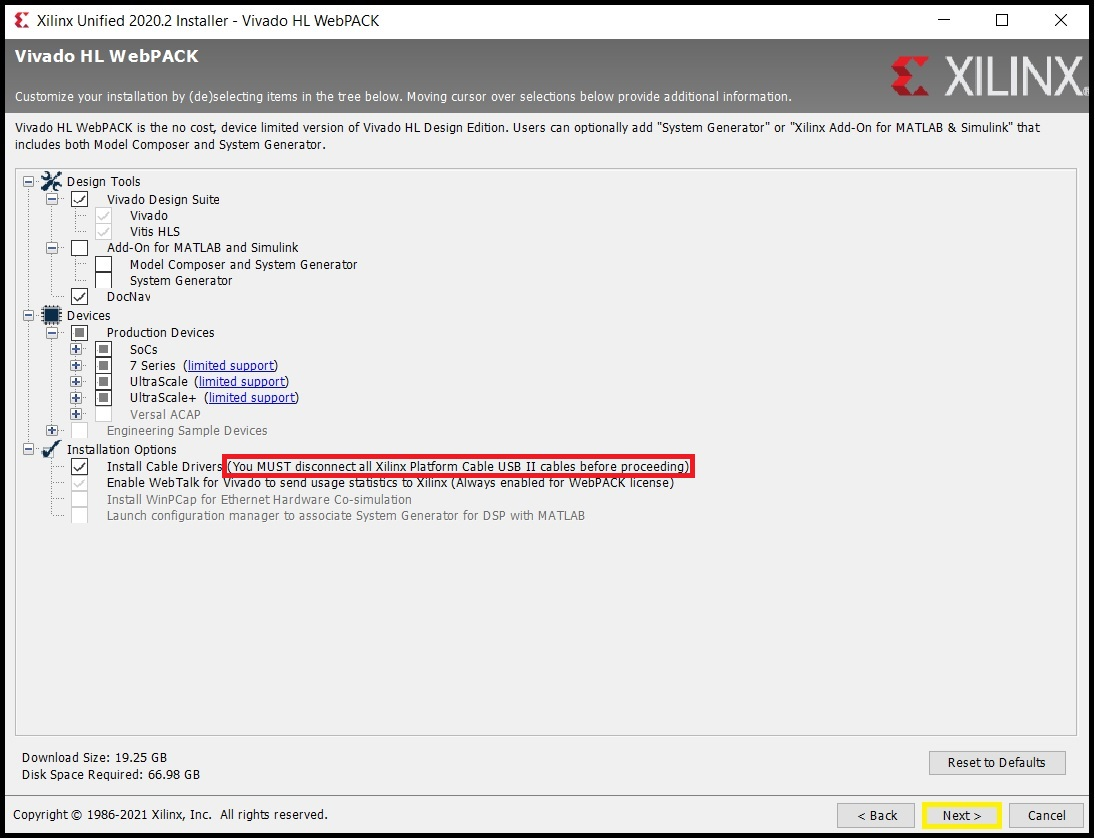
\includegraphics[width=0.7\linewidth]{images/VivadoInstimg012.png}
  \end{center}
  Warning: As stated, disconnect any USB cable that would be connected to your PC from the Nexys board.
\end{minipage}

\begin{minipage}{\linewidth}
  Agree with all the End User Licence Agreement and Terms and conditions and click on "Next".
  \\
  \begin{center}
    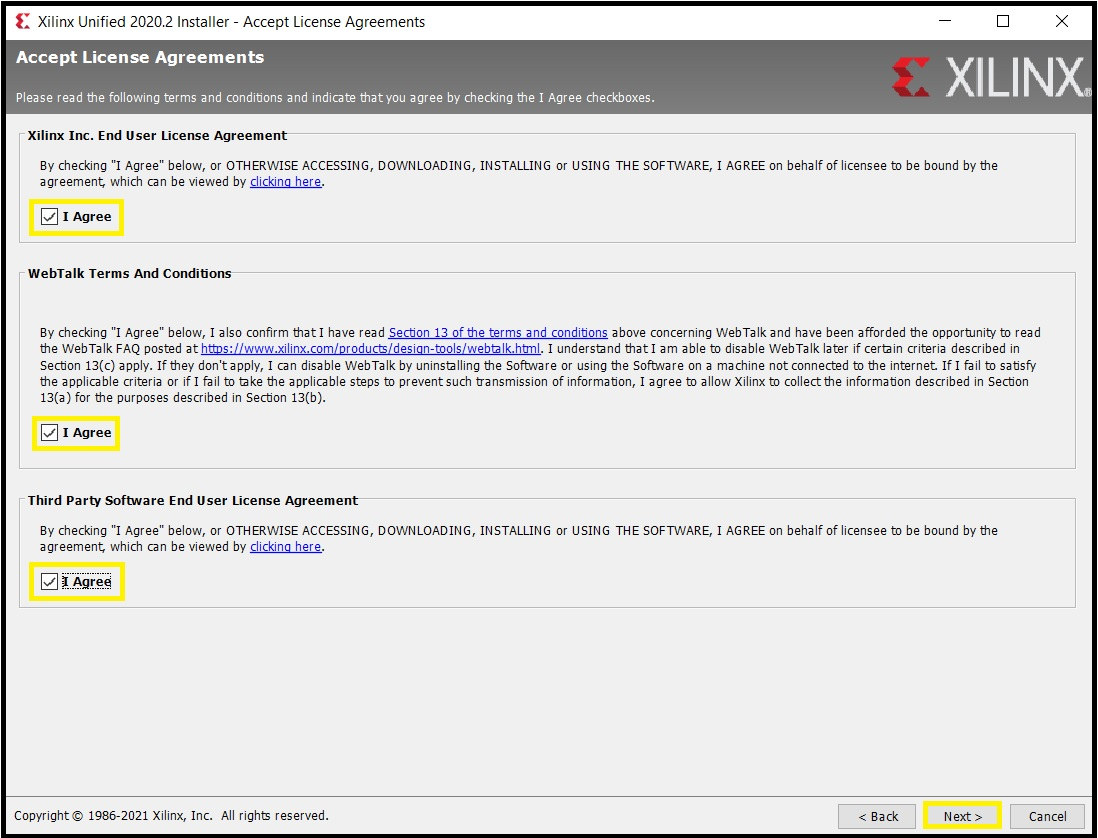
\includegraphics[width=0.7\linewidth]{images/VivadoInstimg013.jpg}
  \end{center}
\end{minipage}

\begin{minipage}{\linewidth}
  Choose the location where you want to install the software and click on "Next".
  \\
  \begin{center}
    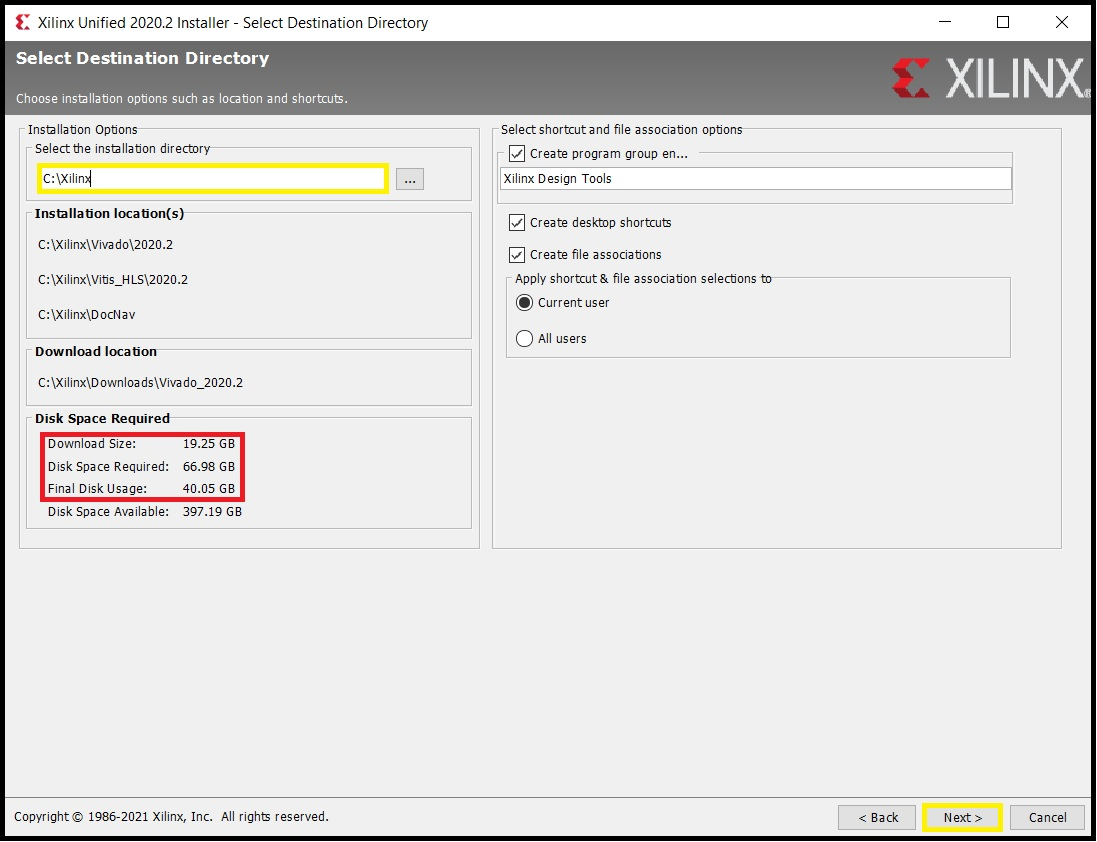
\includegraphics[width=0.7\linewidth]{images/VivadoInstimg014.jpg}
  \end{center}
  Warning : You are about to download 20GB of software and you need 70GB to perform the installation.
\end{minipage}

\begin{minipage}{\linewidth}
  Click on "Yes"
  \\
  \begin{center}
    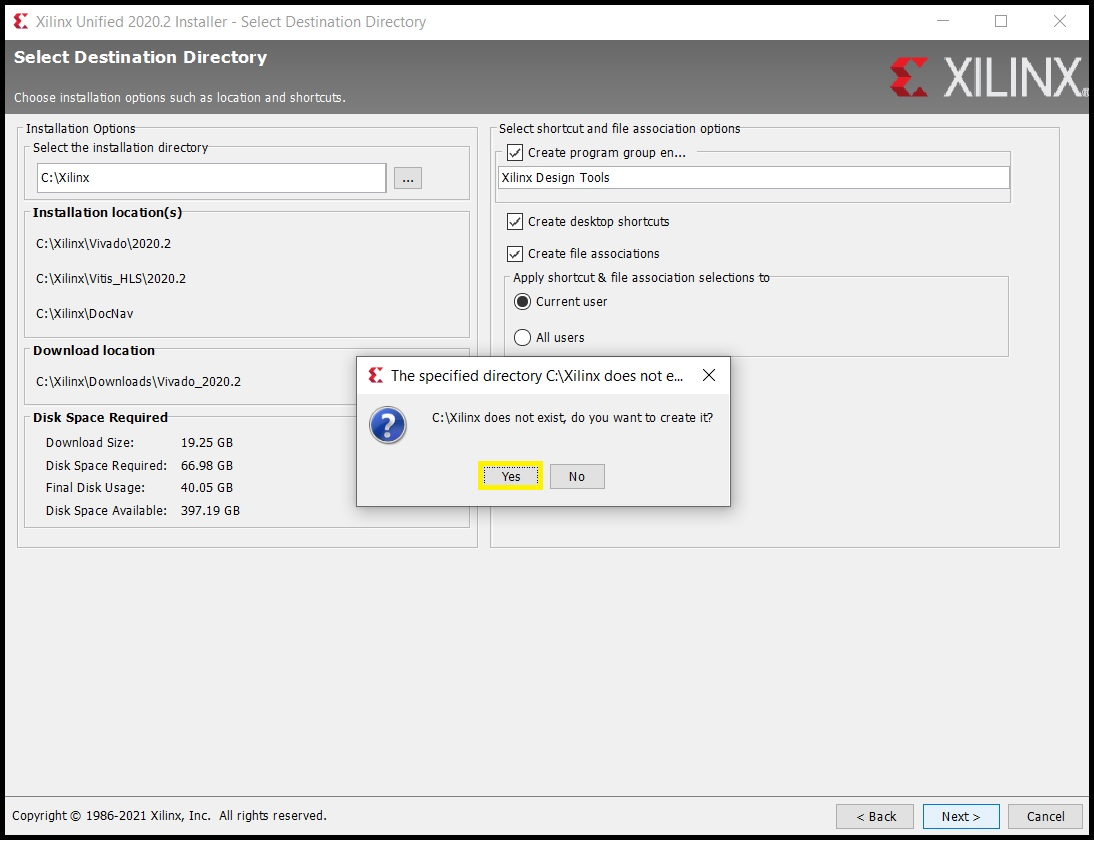
\includegraphics[width=0.7\linewidth]{images/VivadoInstimg015.jpg}
  \end{center}
\end{minipage}

\begin{minipage}{\linewidth}
  Click on "Install"
  \\
  \begin{center}
    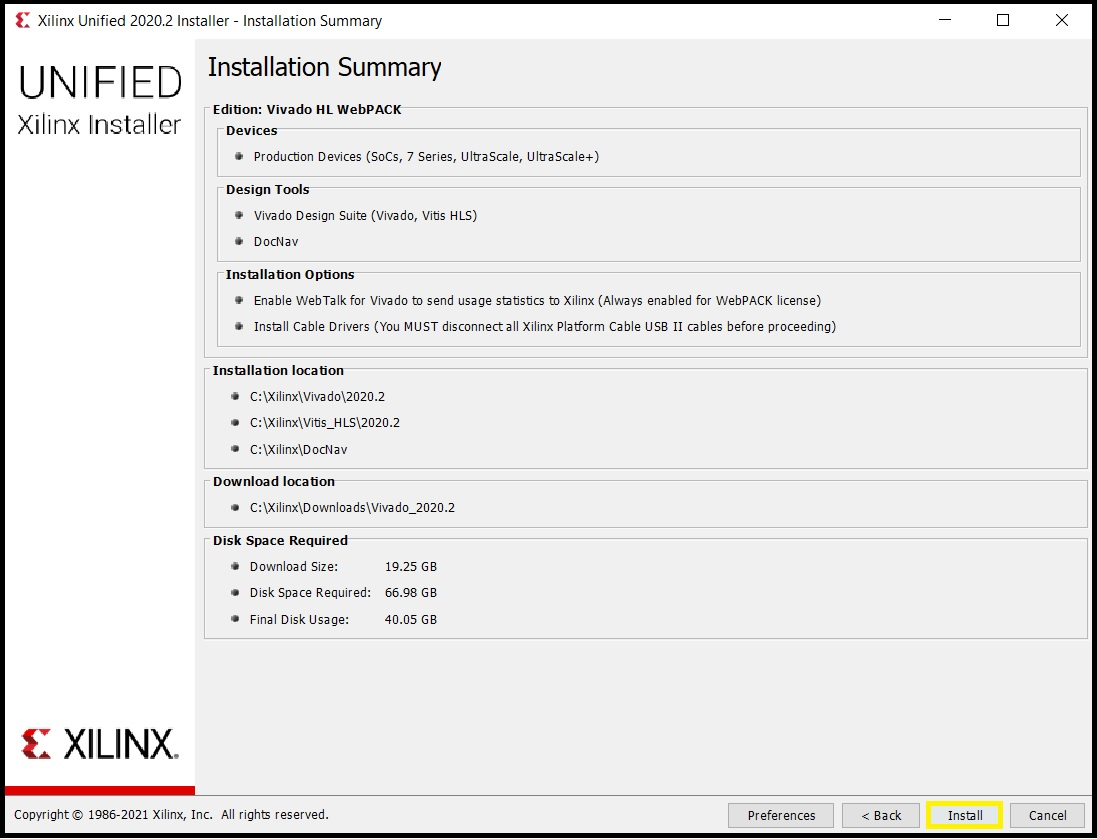
\includegraphics[width=0.7\linewidth]{images/VivadoInstimg016.jpg}
  \end{center}
\end{minipage}

\begin{minipage}{\linewidth}
  Wait for the installation to complete. At the very end of the installation you will be asked if you want
  to install Xilinx device software.
  \\
  \begin{center}
    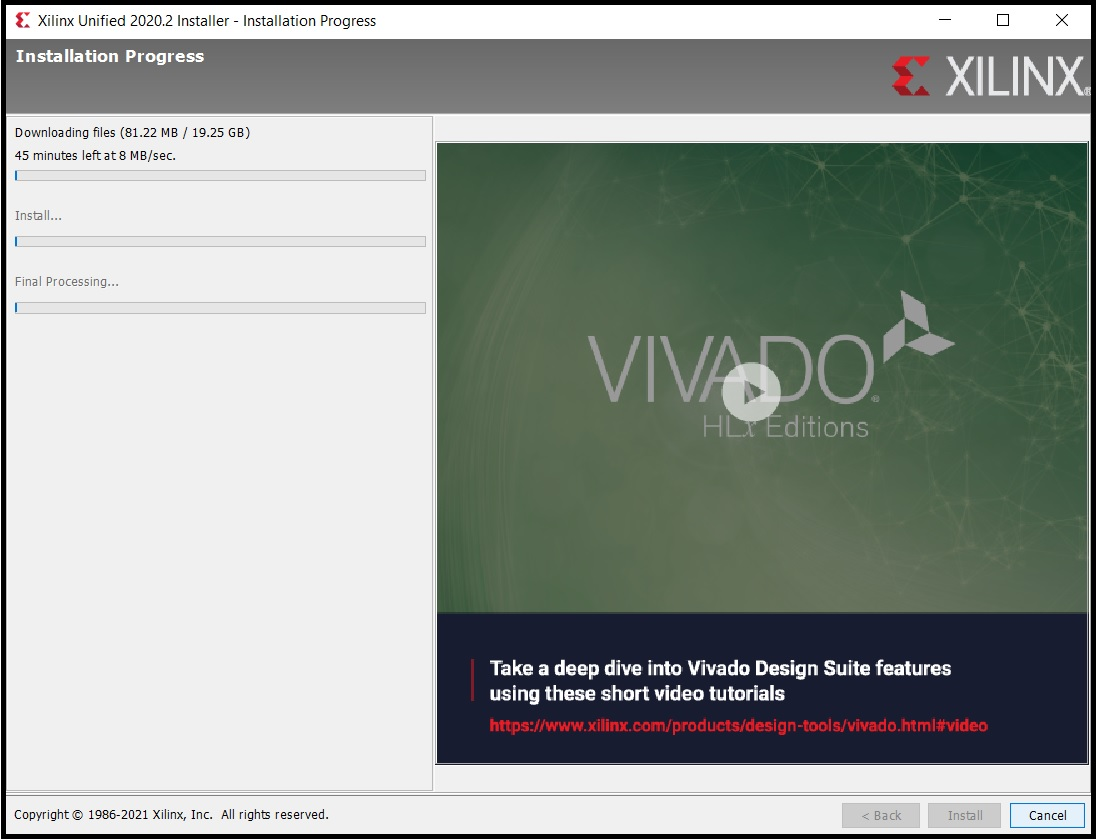
\includegraphics[width=0.7\linewidth]{images/VivadoInstimg017.jpg}
  \end{center}
\end{minipage}

\begin{minipage}{\linewidth}
  Click on "Install"
  \\
  \begin{center}
    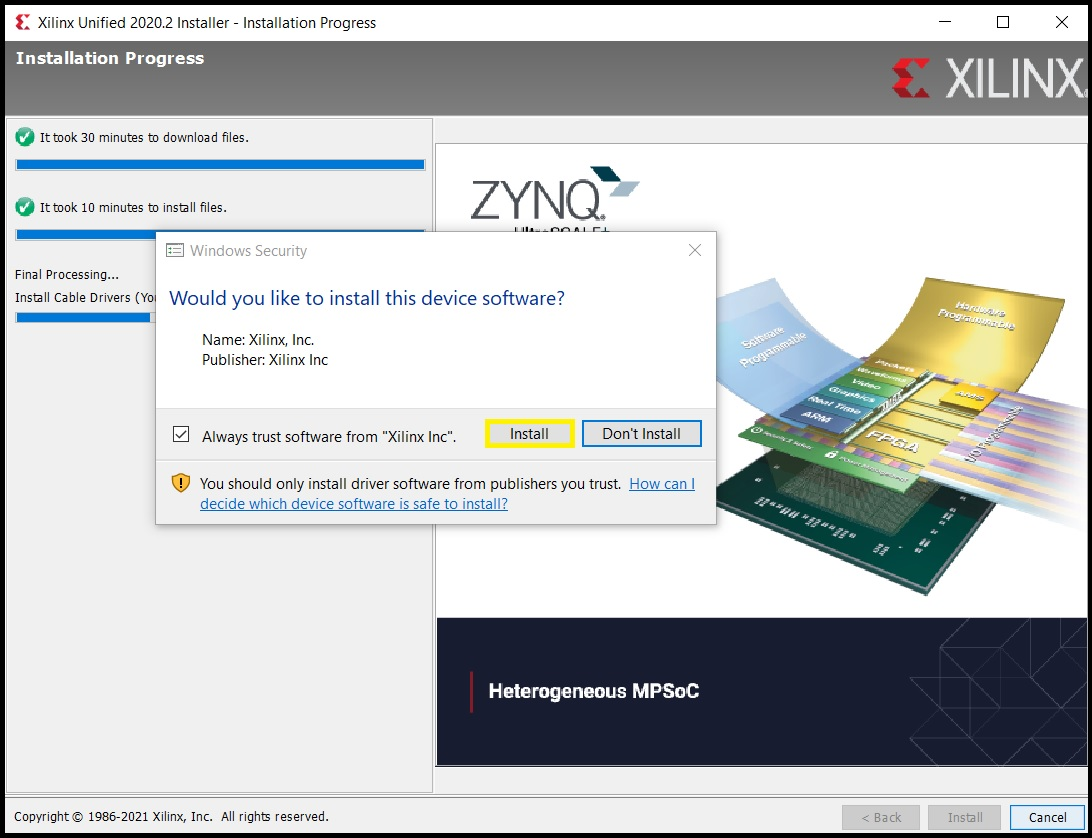
\includegraphics[width=0.7\linewidth]{images/VivadoInstimg018.jpg}
  \end{center}
  Let the installation complete.
\end{minipage}

\begin{minipage}{\linewidth}
  The installation is completed. Click on "OK"
  \\
  \begin{center}
    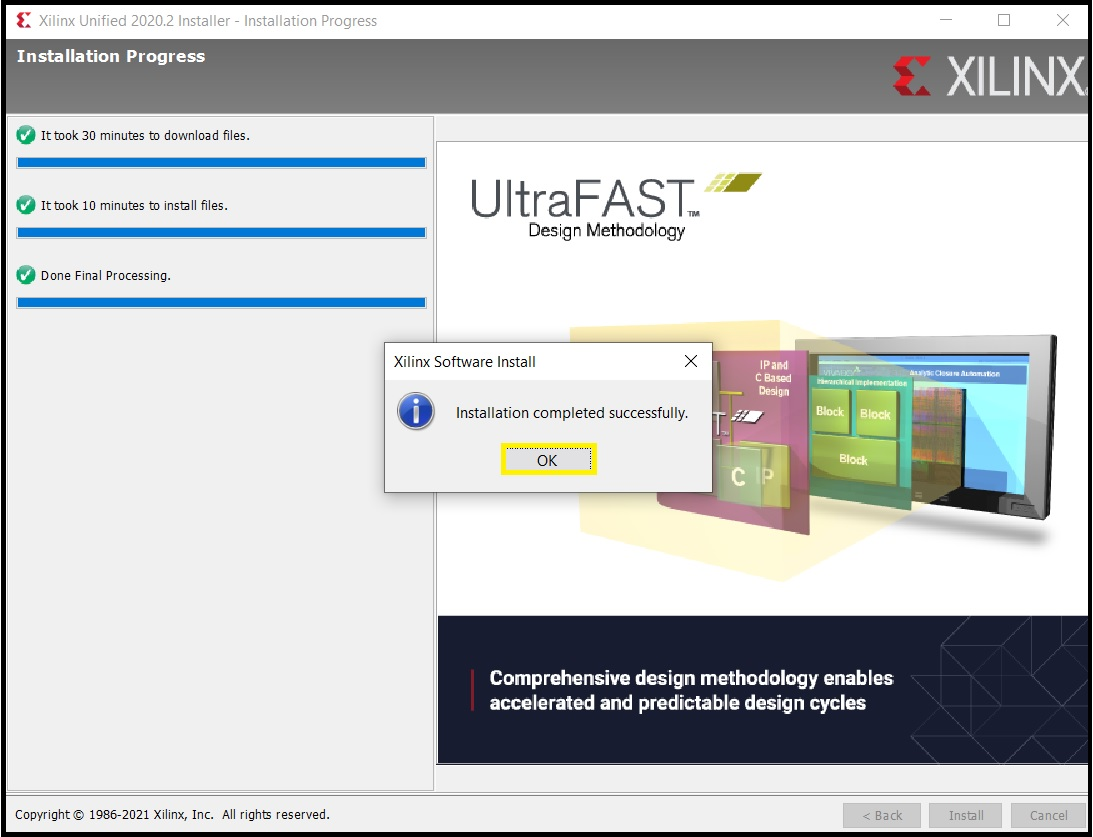
\includegraphics[width=0.7\linewidth]{images/VivadoInstimg019.jpg}
  \end{center}
\end{minipage}

\begin{minipage}{\linewidth}
  You end up with the following icons on your desktop:
  \\
  \begin{center}
    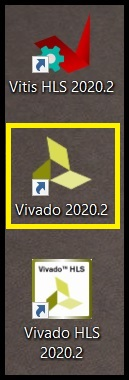
\includegraphics[width=0.2\linewidth]{images/VivadoInstimg020.jpg}
  \end{center}
  Note: Ubuntu users might need to install one missing dependency with: {\tt sudo apt install libtinfo5}
\end{minipage}

\begin{minipage}{\linewidth}
  Launch Vivado 2020.2
  \\
  \begin{center}
    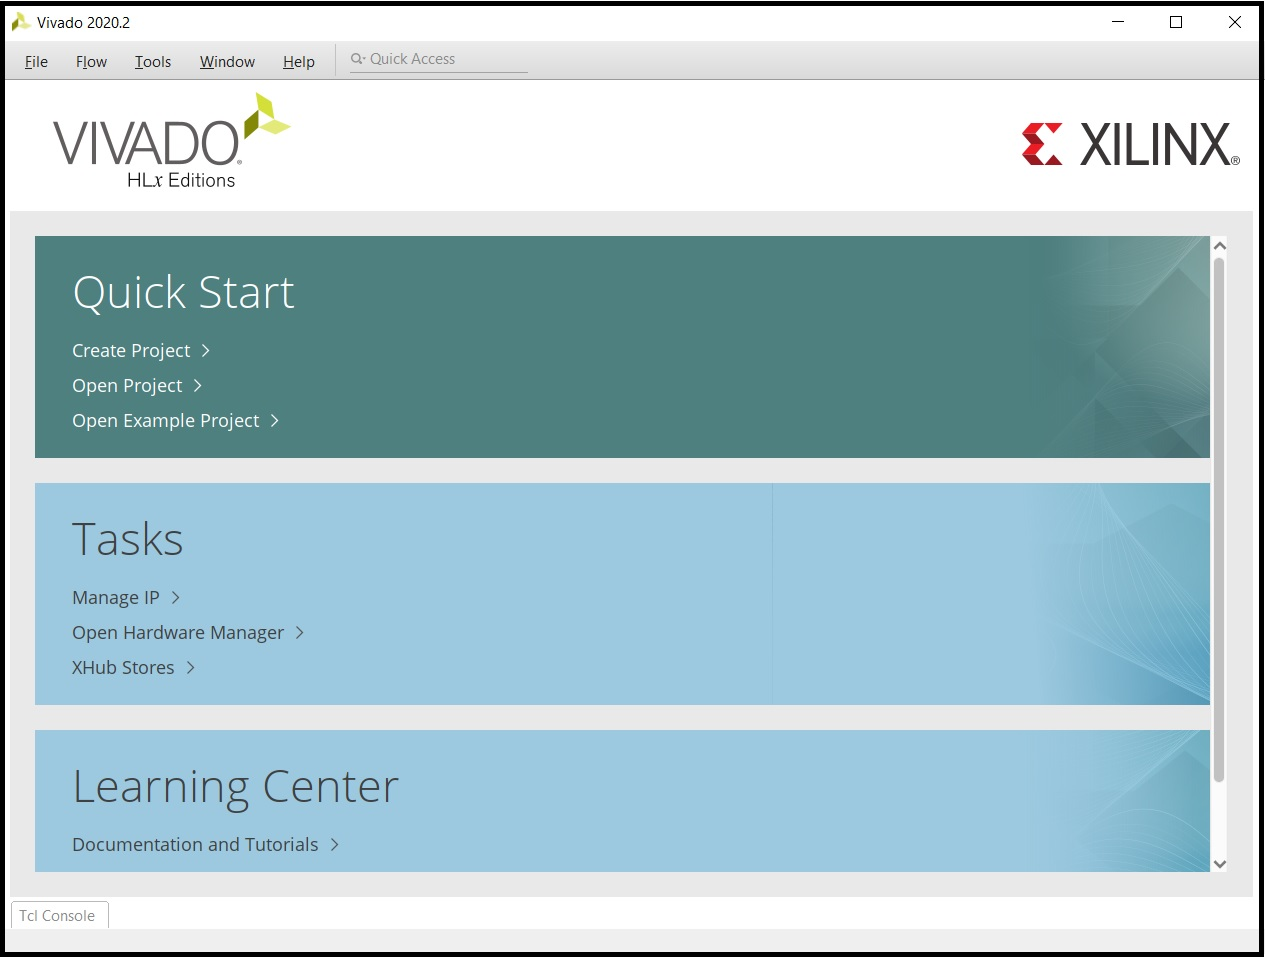
\includegraphics[width=0.7\linewidth]{images/VivadoInstimg021.jpg}
  \end{center}
\end{minipage}

\begin{minipage}{\linewidth}
  Click on "Help"->"Obtain a licence Key"
  \\
  \begin{center}
    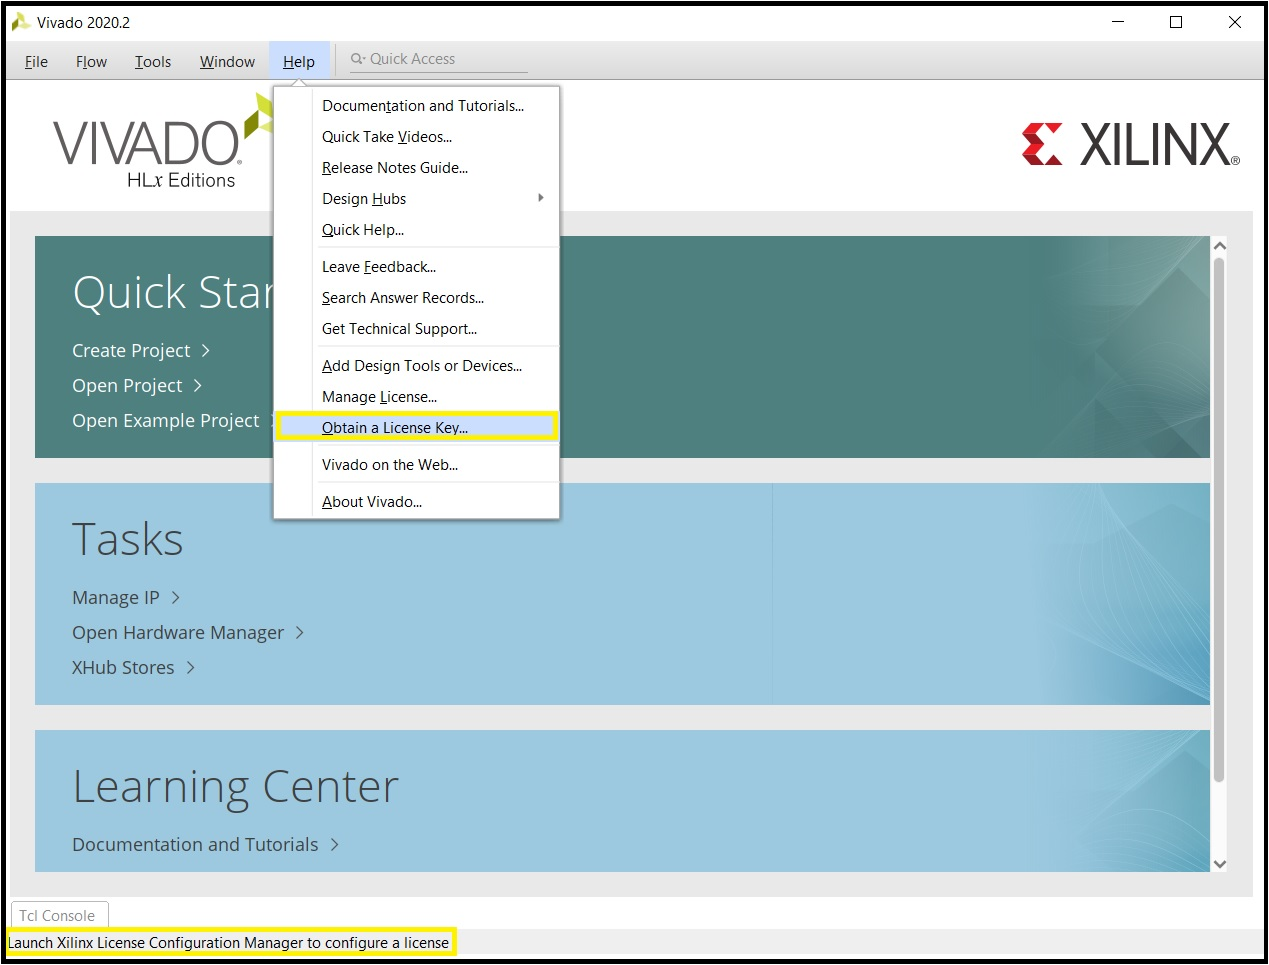
\includegraphics[width=0.7\linewidth]{images/VivadoInstimg022.jpg}
  \end{center}
\end{minipage}

\begin{minipage}{\linewidth}
This launches the Vivado licence manager \\
  \\
  Select "Get Free ISE WebPACK, ISE/Vivado IP or PetaLinux Licenses" \\
  \\
  Click on "Connect Now"
  \\
  \begin{center}
    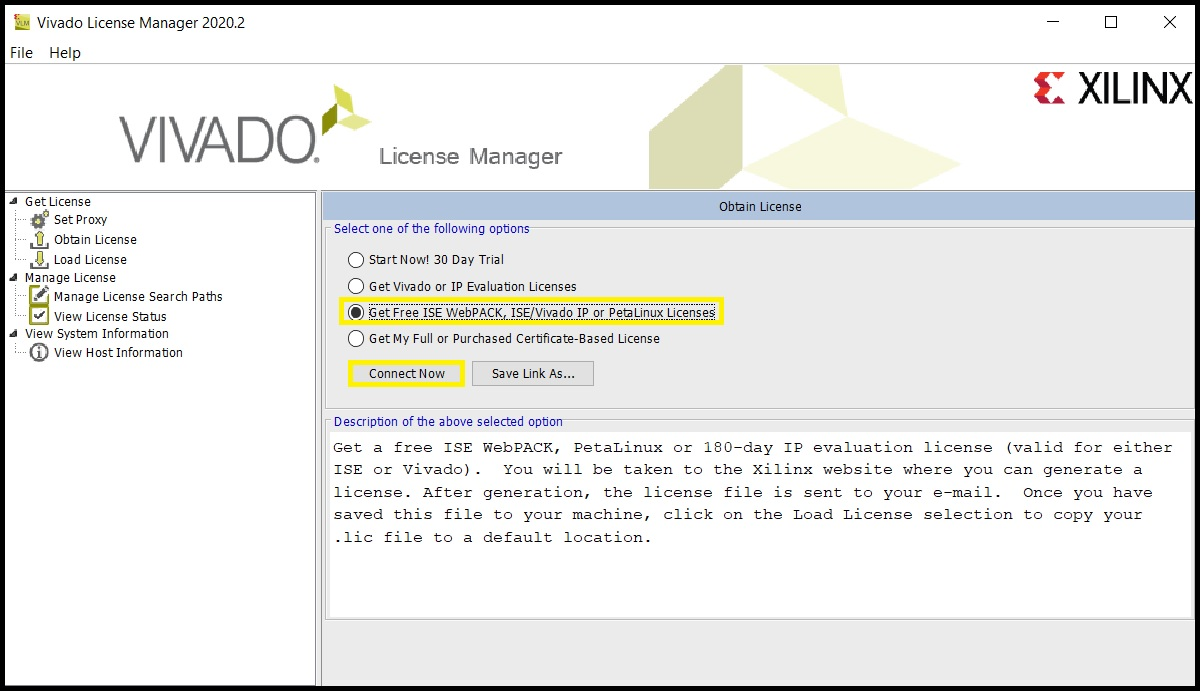
\includegraphics[width=\linewidth]{images/VivadoInstimg023.jpg}
  \end{center}
\end{minipage}

\begin{minipage}{\linewidth}
  Connect with the user account you have created to be able to download the Vivado software.
  If you were not already connected to Xilinx website, this will take you to the main webpage.
  Go back in the licence manager (which is not closed)
  \\
  \begin{center}
    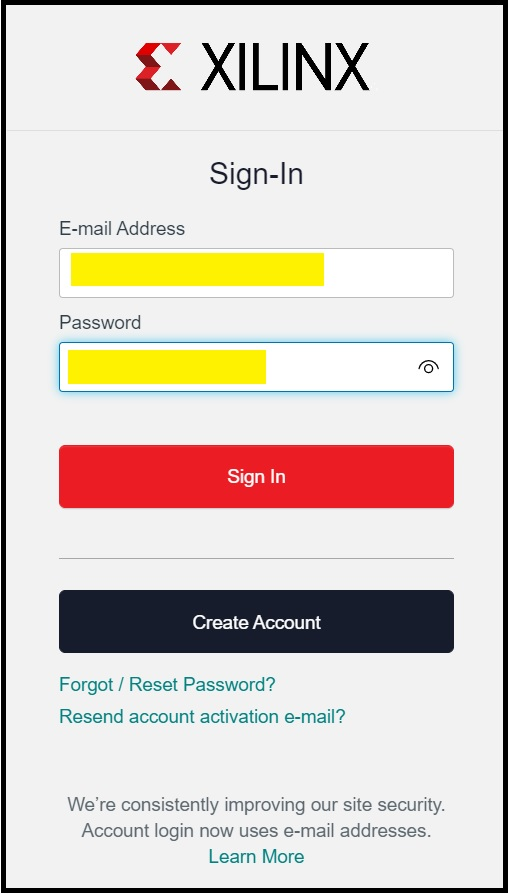
\includegraphics[width=0.3\linewidth]{images/VivadoInstimg024.jpg}
  \end{center}
\end{minipage}

\begin{minipage}{\linewidth}
  Click again on "Connect Now" (ensure "Get Free ISE WebPACK, ISE/Vivado IP or PetaLinux Licenses" is still selected)
  \\
  \begin{center}
    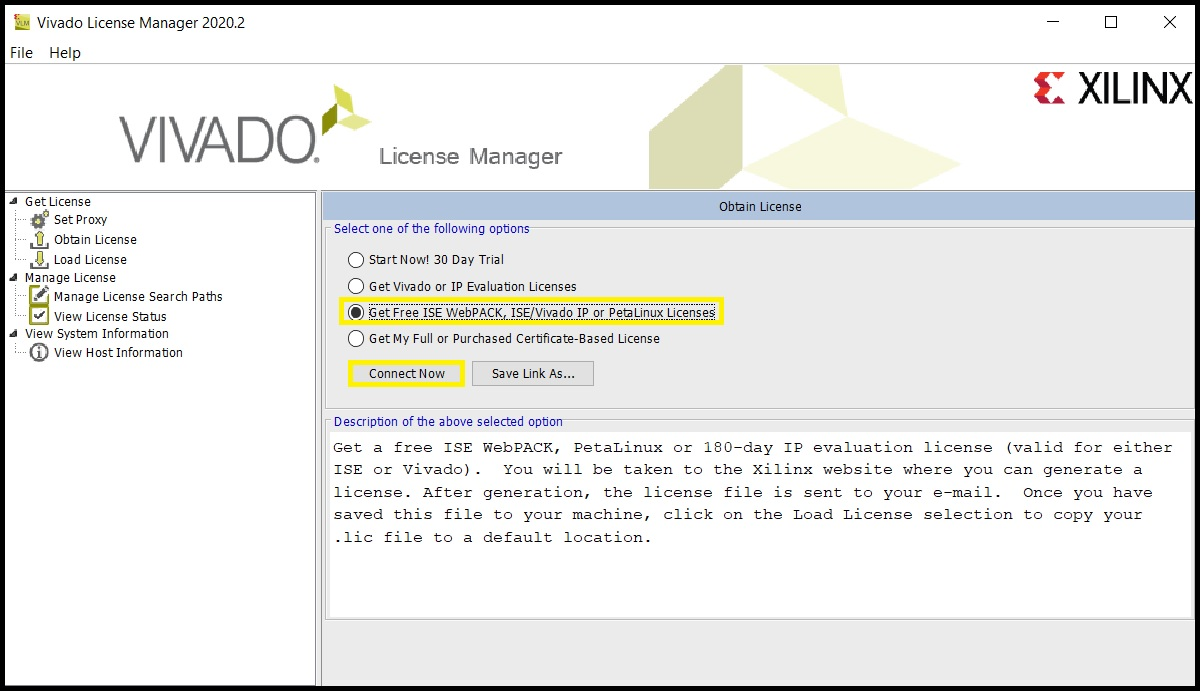
\includegraphics[width=\linewidth]{images/VivadoInstimg023.jpg}
  \end{center}
\end{minipage}

\begin{minipage}{\linewidth}
  You then register your personal information on the Vivado website, and click on "Next".
  \\
  \begin{center}
    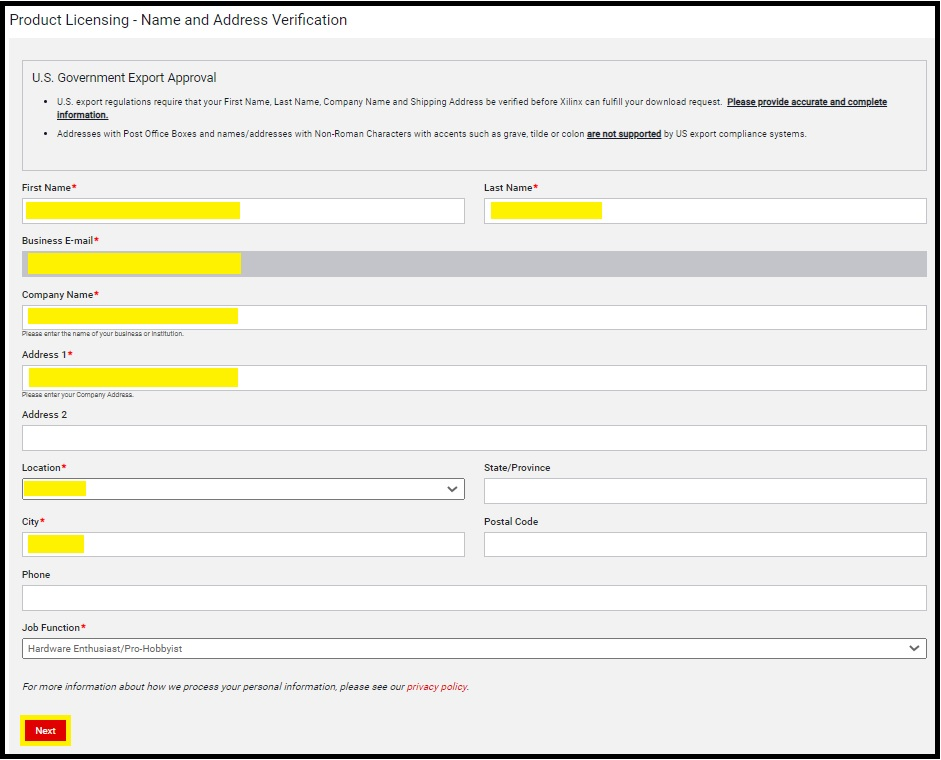
\includegraphics[width=0.7\linewidth]{images/VivadoInstimg025.jpg}
  \end{center}
\end{minipage}


\begin{minipage}{\linewidth}
Select "ISE WebPACK Licence" and "Vivado Design Suite: HL WebPACK 2015 and Earlier License" \\
\\
Then click on "Generate Node-Locked Licence"
\\
\begin{center}
  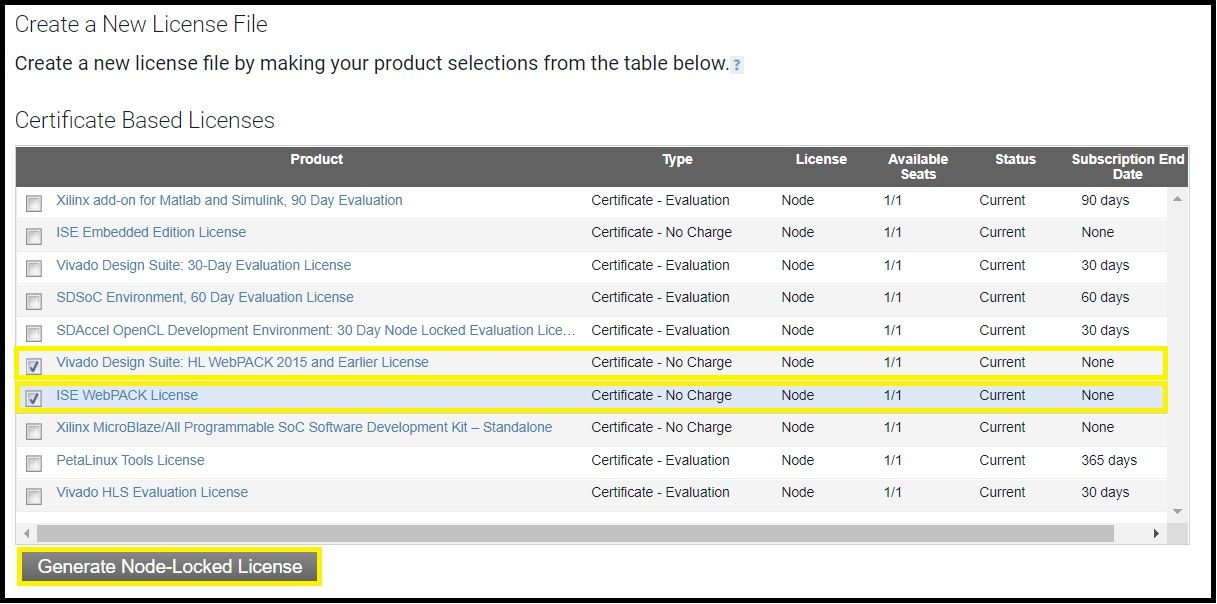
\includegraphics[width=\linewidth]{images/VivadoInstimg026.jpg}
\end{center}
\end{minipage}

\begin{minipage}{\linewidth}
  Click on "Next"
  \\
  \begin{center}
    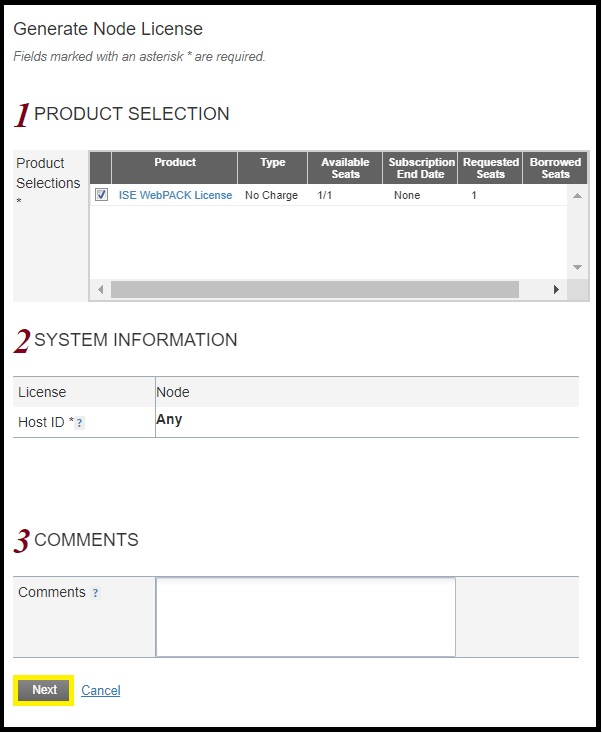
\includegraphics[width=0.5\linewidth]{images/VivadoInstimg027.jpg}
  \end{center}
\end{minipage}

\begin{minipage}{\linewidth}
  Click on "Next"
  \\
  \begin{center}
    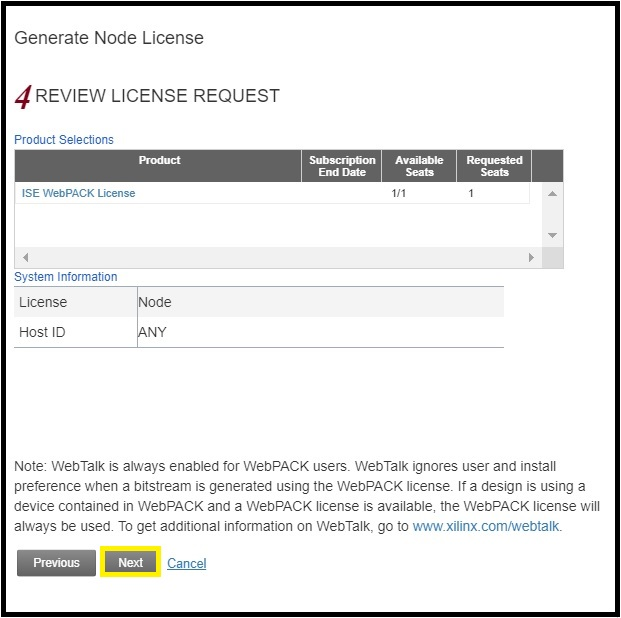
\includegraphics[width=0.5\linewidth]{images/VivadoInstimg028.jpg}
  \end{center}
\end{minipage}


\begin{minipage}{\linewidth}
  Check your email box : You should have received an email from Xilinx, Inc. with a licence file attached and named "Xilinc.lic". \\
  \\
  Retrieve this file on your PC and keep it in safe place.
  \\
  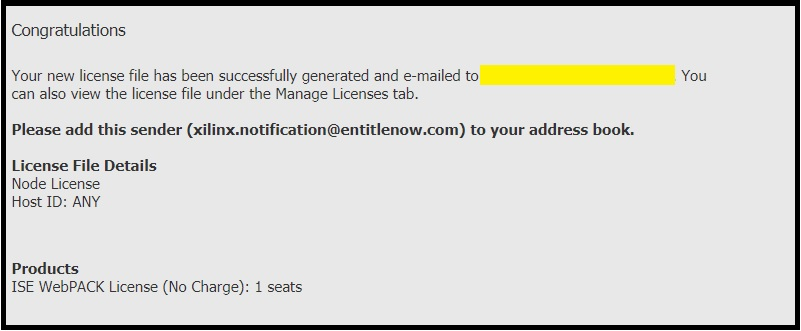
\includegraphics[width=\linewidth]{images/VivadoInstimg029.jpg}
\end{minipage}

\begin{minipage}{\linewidth}
  Go back to the licence manager (which is still running). \\
  \\
  Set "Load License" and click on "Copy License"
  \\
  \begin{center}
    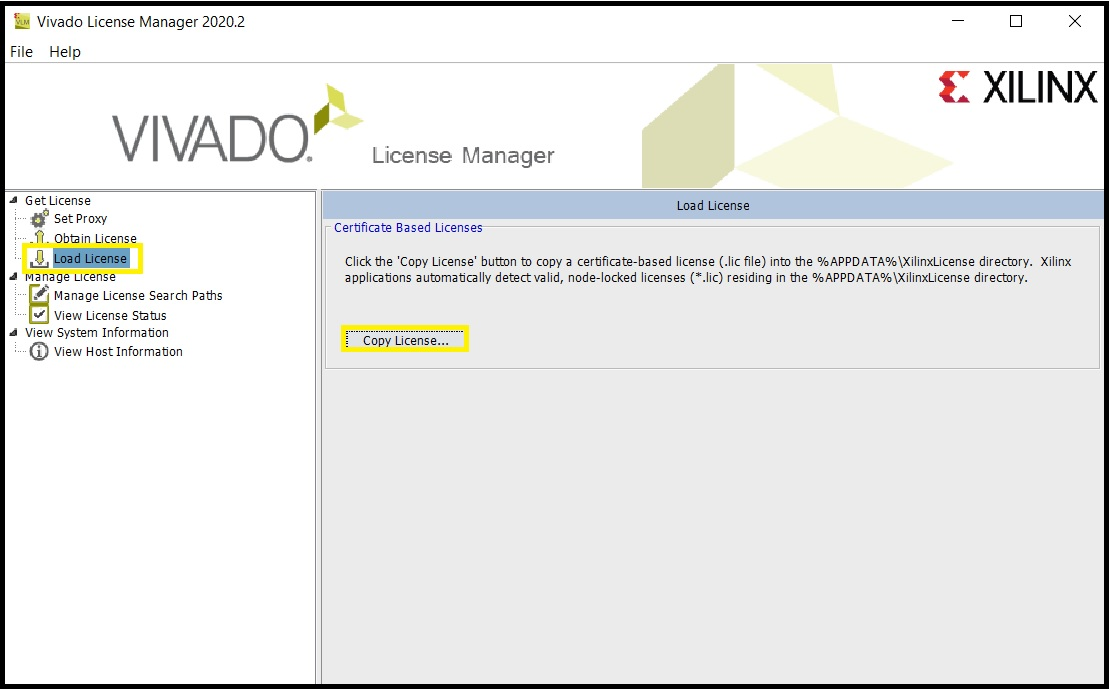
\includegraphics[width=0.8\linewidth]{images/VivadoInstimg030.jpg}
  \end{center}
\end{minipage}

\begin{minipage}{\linewidth}
  Browse to the location where you saved "Xilinc.lic" file, select it and click on "Open".
  \\
  \begin{center}
    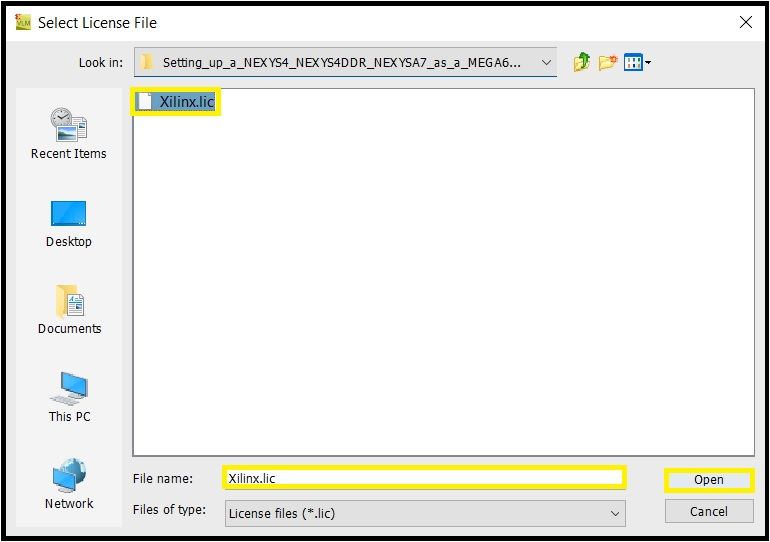
\includegraphics[width=0.7\linewidth]{images/VivadoInstimg031.jpg}
  \end{center}
\end{minipage}

\begin{minipage}{\linewidth}
  Click on "OK" and close the Vivado licence manager.
  \\
  \begin{center}
    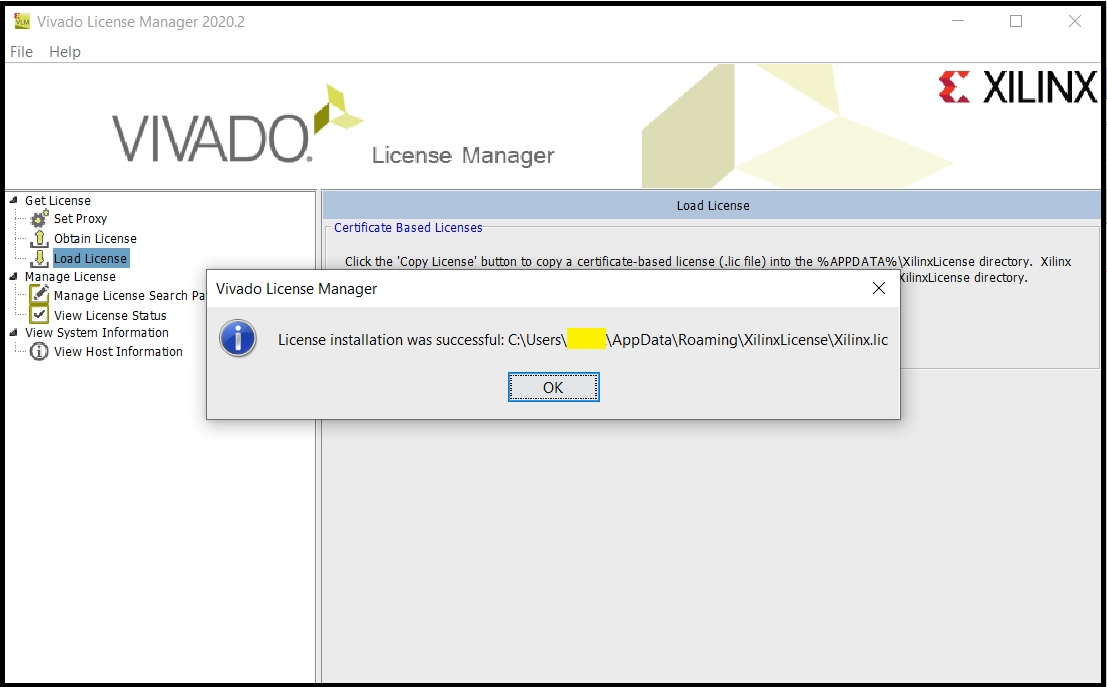
\includegraphics[width=0.7\linewidth]{images/VivadoInstimg032.jpg}
  \end{center}

  Your Vivado software is registered and you can now use it.
\end{minipage}

\section{Installing the FTDI drivers}

The FTDI drivers are needed in order for your PC to communicate with the hardware's JTAG port and serial comms port (note that the single physical USB connection made to your PC actually provides these two ports).

\subsection{Linux drivers}

Some Linux users have reported that they have found the FTDI drivers to be installed within their Linux distributions out-of-the-box, while others have found they needed to run this extra command after installing Vivado:

cd /opt/Xilinx/Vivado/2018.3/data/xicom/cable\_drivers/lin64/install\_script/install\_drivers \\
sudo ./install\_drivers

\subsection{Windows drivers}

Download the following archive to install the drivers:

\begin{itemize}
  \item \url{https://www.ftdichip.com/Drivers/CDM/CDM21228\_Setup.zip}
\end{itemize}

Unzip the file \textbf{CDM21228\_Setup.zip}, you get the file \textbf{CDM21228\_Setup.exe}.

\textcolor{red}{\underline{Warning}: \\
Before installing the drivers, it is imperative to switch off the Nexys4 board and to disconnect the USB cable from the PC.}

\begin{minipage}{\linewidth}
  Review the devices already installed before the installation:
  \\
  \begin{center}
    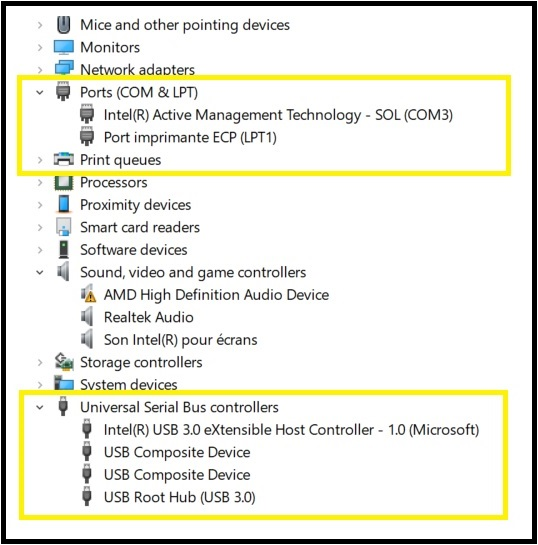
\includegraphics[width=0.6\linewidth]{images/img001_install_drivers_00.jpg}
  \end{center}
\end{minipage}

\begin{minipage}{\linewidth}
  Run the file CDM21228\_Setup.exe as administrator:
  \\
  \begin{center}
    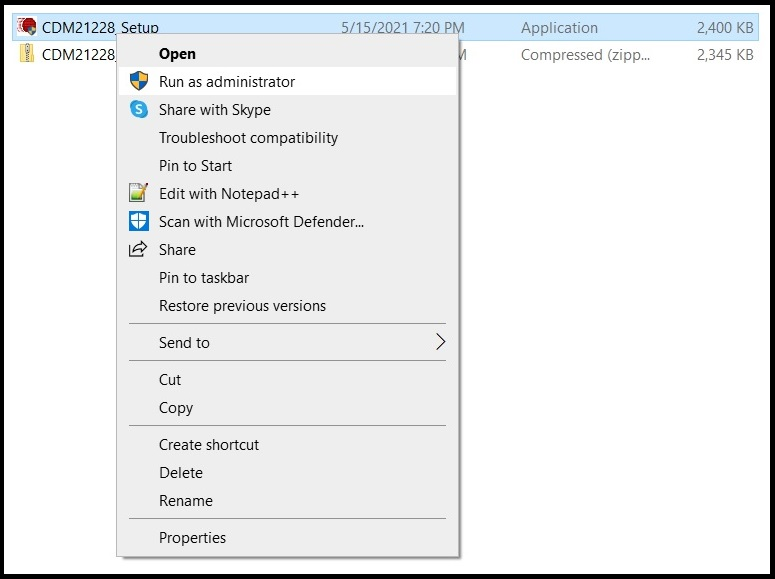
\includegraphics[width=0.6\linewidth]{images/img001_install_drivers_01.jpg}
  \end{center}
\end{minipage}

Confirm that you want to run the program.

\begin{minipage}{\linewidth}
  Click on "Extract".
  \\
  \begin{center}
    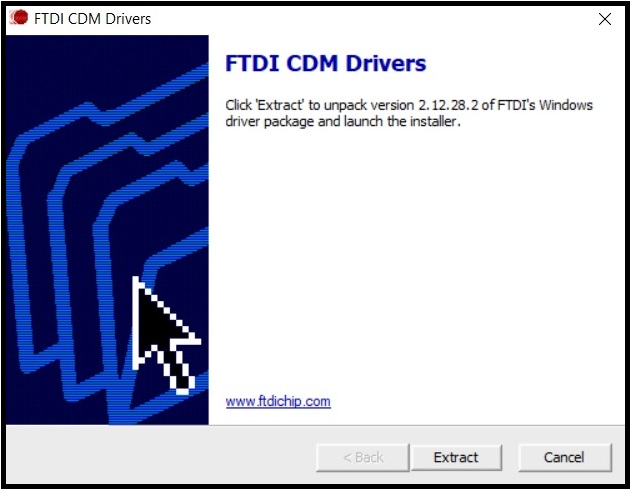
\includegraphics[width=0.6\linewidth]{images/img001_install_drivers_02.jpg}
  \end{center}
\end{minipage}

\begin{minipage}{\linewidth}
  Click on "Next >"
  \\
  \begin{center}
    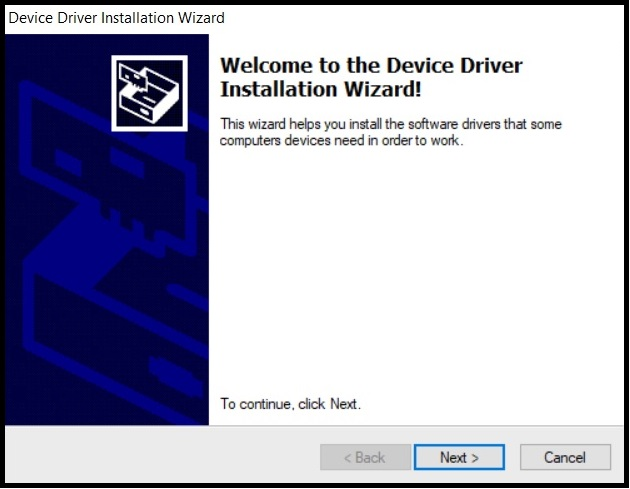
\includegraphics[width=0.6\linewidth]{images/img001_install_drivers_03.jpg}
  \end{center}
\end{minipage}

\begin{minipage}{\linewidth}
  Accept the agreement and click on "Next >".
  \\
  \begin{center}
    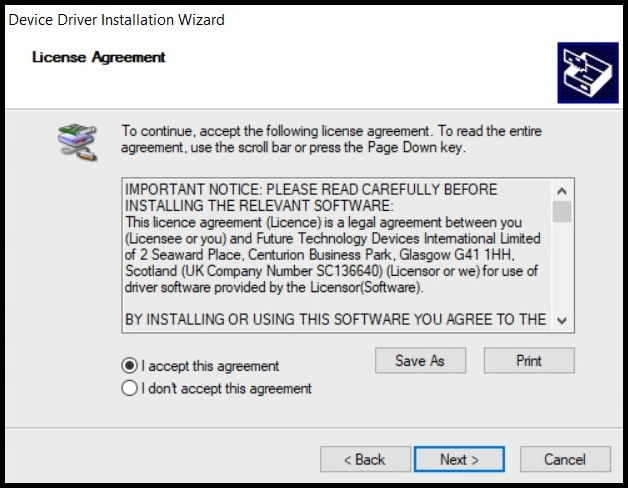
\includegraphics[width=0.6\linewidth]{images/img001_install_drivers_04.jpg}
  \end{center}
\end{minipage}

The installation of the drivers starts.

\begin{minipage}{\linewidth}
  Click on "Finish".
  \\
  \begin{center}
    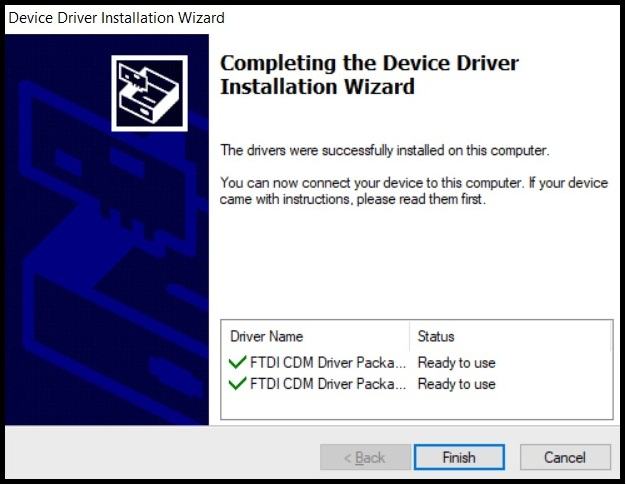
\includegraphics[width=0.6\linewidth]{images/img001_install_drivers_05.jpg}
  \end{center}
\end{minipage}

Connect the USB cable to a USB port on the PC \textcolor{red}{without turning on the Nexys4 board}.

Connecting the USB cable triggers the appearance of new devices.

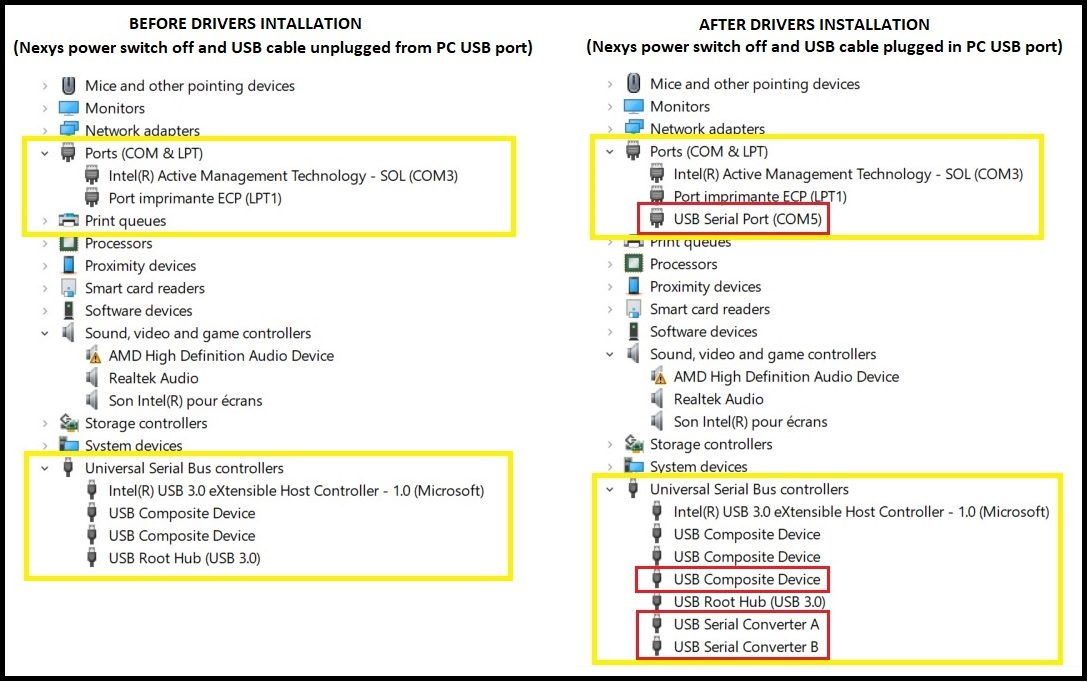
\includegraphics[width=\linewidth]{images/img001_install_drivers_07.jpg}

\begin{itemize}
  \item An additional COM port has been installed: \textcolor{red}{This is the COM port that will be used to communicate with the Nexys4 board.}
  \item An additional USB composite device has been installed.
  \item Two USB serial converter devices have been installed.
\end{itemize}

At this point the Nexys4 board has still not been powered up.

For more information about the installed drivers, you can download the corresponding documentation:

\begin{itemize}
  \item \url{https://ftdichip.com/wp-content/uploads/2020/08/AN\_396-FTDI-Drivers-Installation-Guide-for-Windows-10.pdf}
  \item \url{https://ftdichip.com/wp-content/uploads/2021/01/AN\_119\_FTDI\_Drivers\_Installation\_Guide\_for\_Windows7.pdf}
\end{itemize}

\section{Flashing the main FPGA using Vivado}
\label{sec:mainfpgaflashing}

Firstly, to clarify that when we say 'flashing the FPGA', in reality, what we mean is that we are flashing the QSPI flash memory chip that the FPGA makes use of upon startup in order to quickly load the bitstream from.

The diagram below shows two common pathways that the FPGA can load bitstreams at startup:

\begin{center}
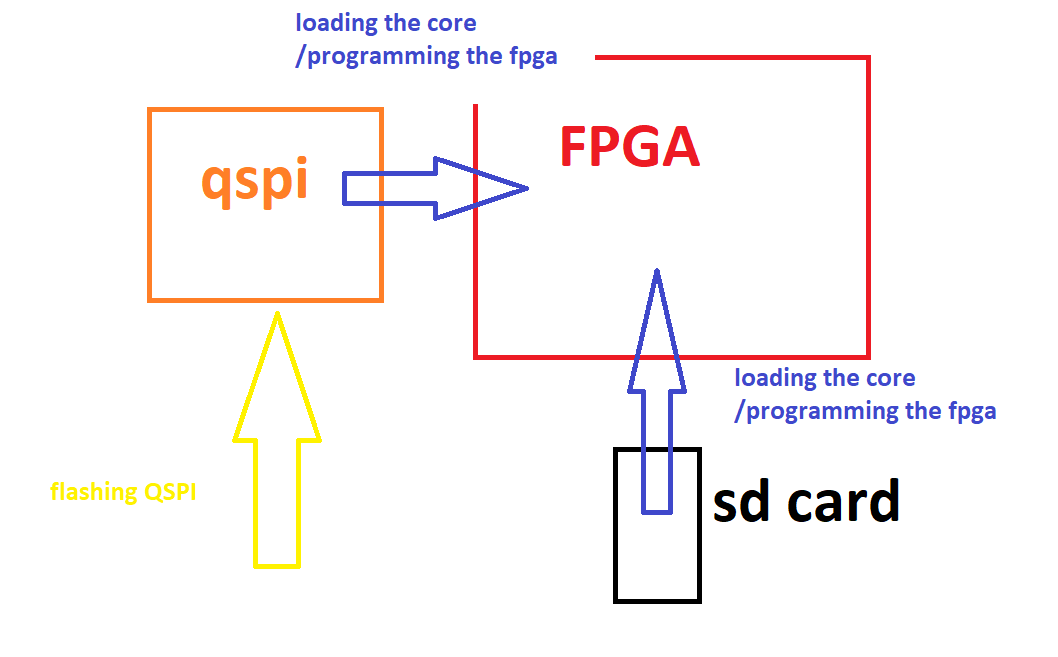
\includegraphics[width=0.8\linewidth]{images/flashing_fpga.png}
\end{center}

\begin{itemize}
  \item We can first flash a bitstream/core-file onto the QSPI flash memory chip, and the FPGA can load this quickly at power-up. Flashing the QSPI is quite slow, but the reward of a fast boot-up time is an advantage.
  \item Nexys board users can drop a bitstream file onto our SD card and let the FPGA load it (somewhat more slowly) from there at power-up. This allows them to swap/upgrade bitstreams quickly without the need for a TE0790-03 JTAG programming module. This feature is planned to be added to the MEGA65 later, though.
\end{itemize}

In this section, we describe the pathway that makes use of the QSPI.

Many of the following steps in this section are applicable not only to MEGA65 R2/R3/R3A/R4 owners, but Nexys4 board owners too. There are a few points of distinction along the way that readers will be made aware of.

If you choose to proceed, you will need a functioning installation of Xilinx's Vivado software, and the FTDI drivers installed, as described in the earlier sections.

You will also need to download or build an .mcs bitstream file (and optional
.prm checksum verification file) that you intend to flash onto the QSPI chip via
Vivado. See
the {\bf MEGA65 Book}
for more details on where such files can be downloaded.

\begin{tcolorbox}[colback=white,coltext=black]
\underline{For MEGA65 R2/R3/R3A/R4 owners}:\\
\\
You will need a TE0790-03 JTAG programming module. It is also necessary to have
dip-switches 1 and 3 in the ON position and dip-switches 2 and 4 in the
OFF position on the TE-0790.
With your MEGA65 disconnected from the power, the TE-0790 must be
installed on the JB1 connector which is located between the floppy data cable and the audio jack.
The gold-plated hole of the TE-0790 must line up with the screw
hole below.  The mini-USB cable will then connect on the side towards the 3.5" floppy drive.
The following image shows the correct position: The TE0790 is surrounded by the yellow box,
and the dip-switches by the red box. Dip-switch 1 is the one nearest the floppy data cable. \\
\\
\includegraphics[width=\linewidth]{images/jtag_detail_02.jpg}
\end{tcolorbox}

\begin{tcolorbox}[colback=white,coltext=black]
\underline{For Nexys4 board owners}: \\
\\
  Simply connect your micro-usb cable between your Nexys4 board and your PC via the port labeled 'PROG UART' (J6), as shown: \\
\\
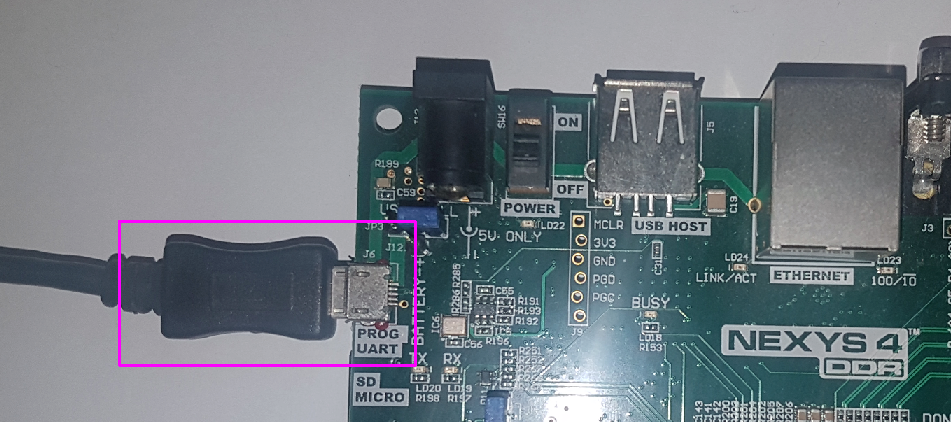
\includegraphics[width=\linewidth]{images/nexys4_comms.png}
\\
\\
Also, set J1 jumper to the QSPI position:
\\
\begin{center}
  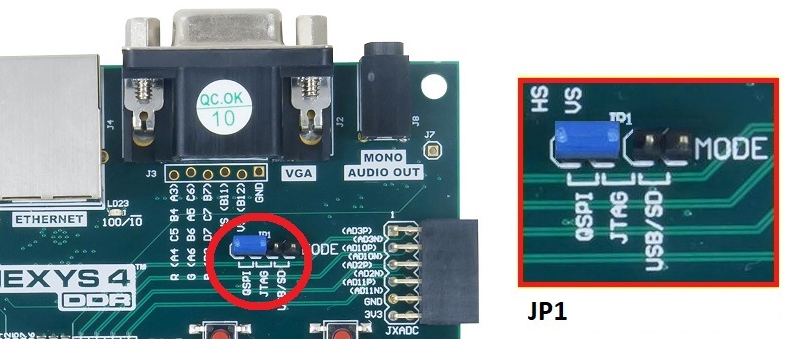
\includegraphics[width=0.8\linewidth]{images/nexys4_j2.png}
\end{center}

\end{tcolorbox}

\begin{itemize}
  \item Connect your non-8-bit computer to the FPGA programming device using the appropriate USB cable.
  \item Switch the MEGA65 computer ON.
  \item Open Vivado.
\end{itemize}


\begin{minipage}{\linewidth}
  Step 1a: Create a new Vivado project with "File", "Project", "New...". \\
  NOTE: On future occasions that you need to flash the QSPI, just re-open this project (no need to create a new project each time).  \\
  \begin{center}
    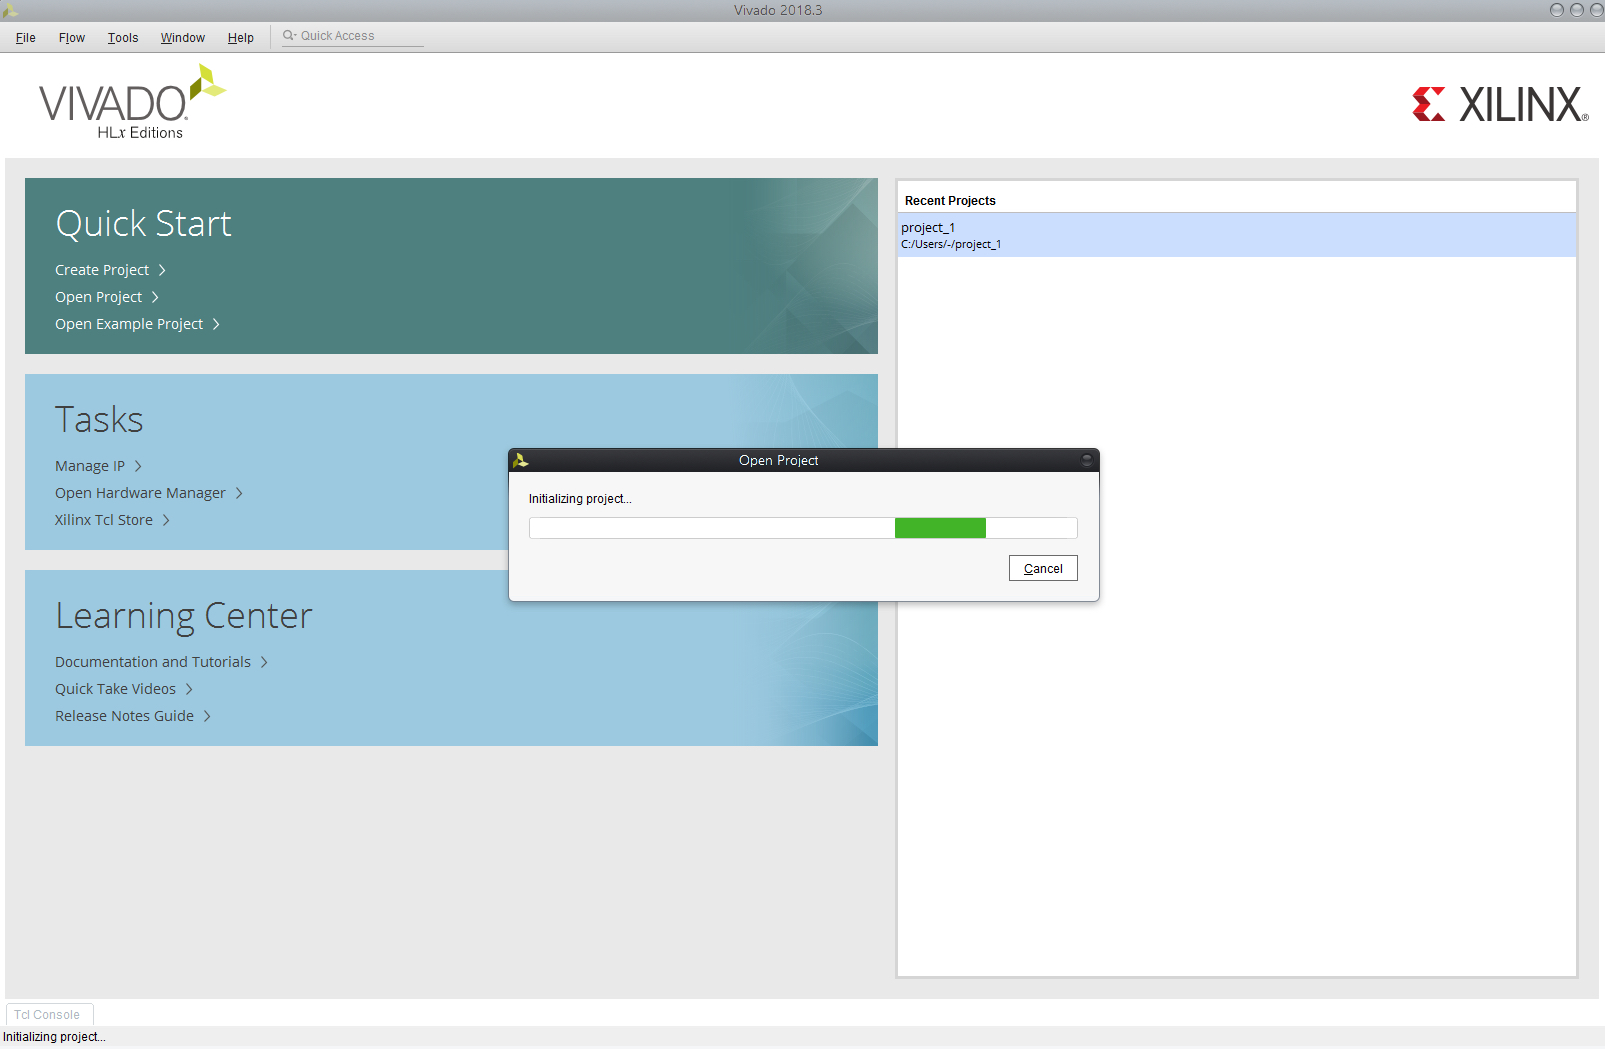
\includegraphics[width=0.8\linewidth]{images/vivado01.png}
  \end{center}
\end{minipage}

\vspace{5mm}

\begin{minipage}{\linewidth}
  Step 1b: The 'New Project' wizard appears. Click on "Next": \\
  \begin{center}
    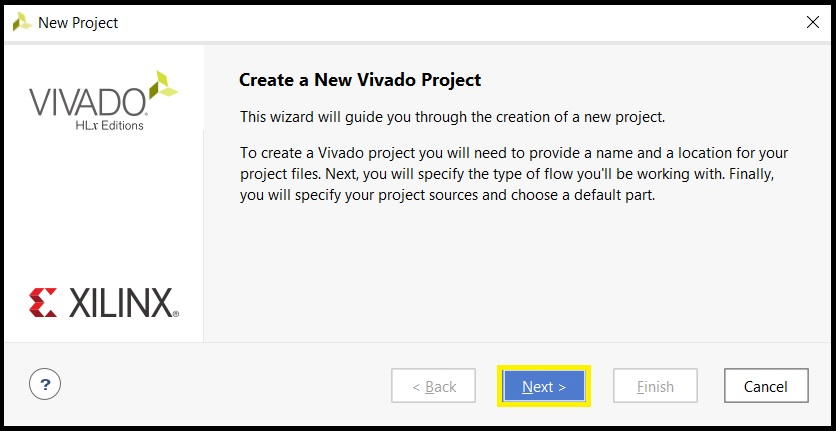
\includegraphics[width=0.8\linewidth]{images/vivado01b.png}
  \end{center}
\end{minipage}

\begin{minipage}{\linewidth}
  Step 1c: Name your project and choose the location you like, then click on "Next":\\
  \begin{center}
    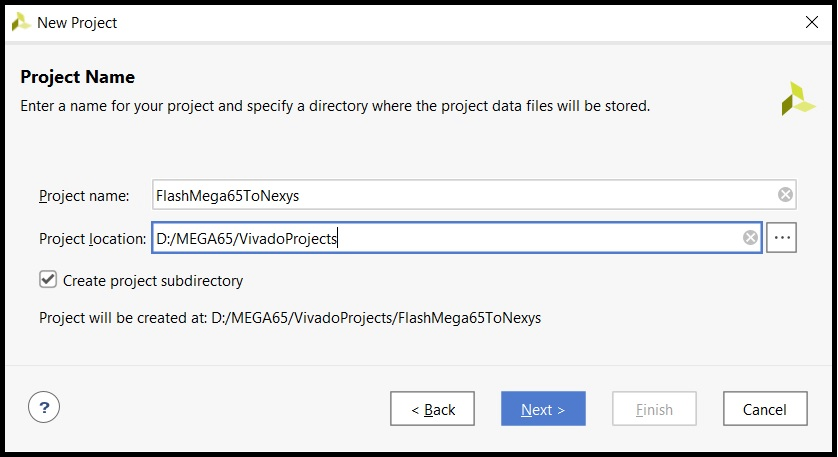
\includegraphics[width=0.8\linewidth]{images/vivado01c.png}
  \end{center}
\end{minipage}

\vspace{5mm}

\begin{minipage}{\linewidth}
  Step 1d: Keep the default selected options and click on "Next": \\
  \begin{center}
    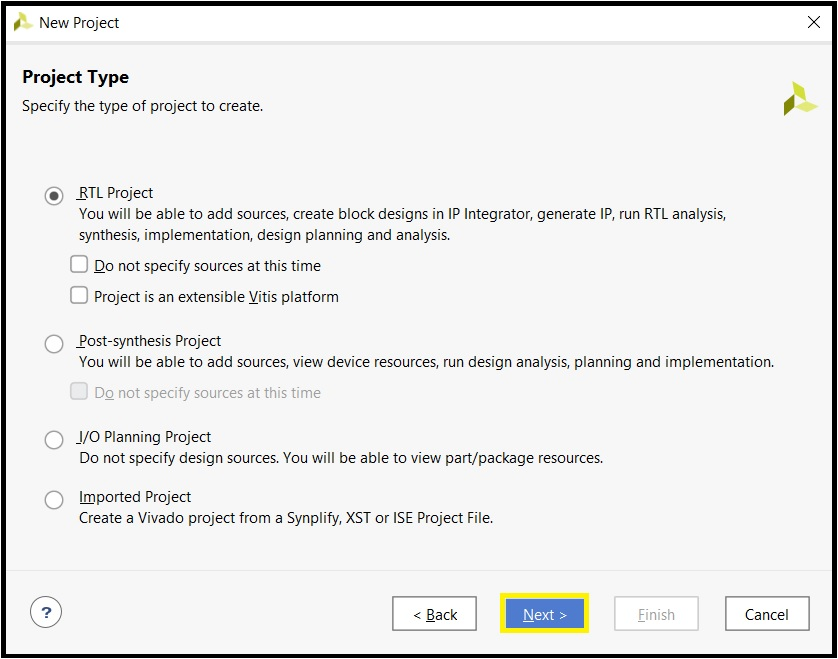
\includegraphics[width=0.8\linewidth]{images/vivado01d.png}
  \end{center}
\end{minipage}

\begin{minipage}{\linewidth}
  Step 1e: Do not add any sources, keep the default selected options and click on "Next": \\
  \begin{center}
    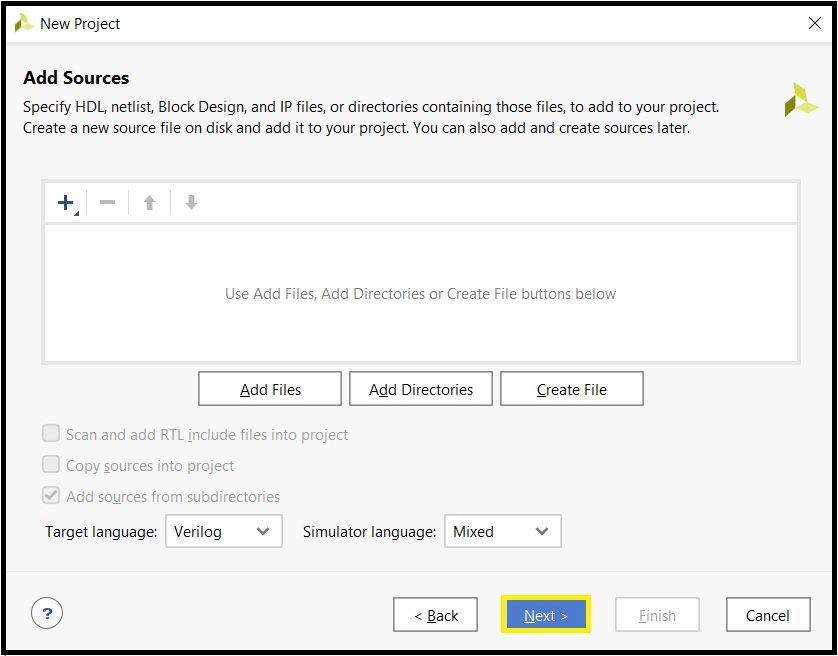
\includegraphics[width=0.7\linewidth]{images/vivado01e.png}
  \end{center}
\end{minipage}

\vspace{5mm}

\begin{minipage}{\linewidth}
  Step 1f: Keep the default selected options and click on "Next": \\
  \begin{center}
    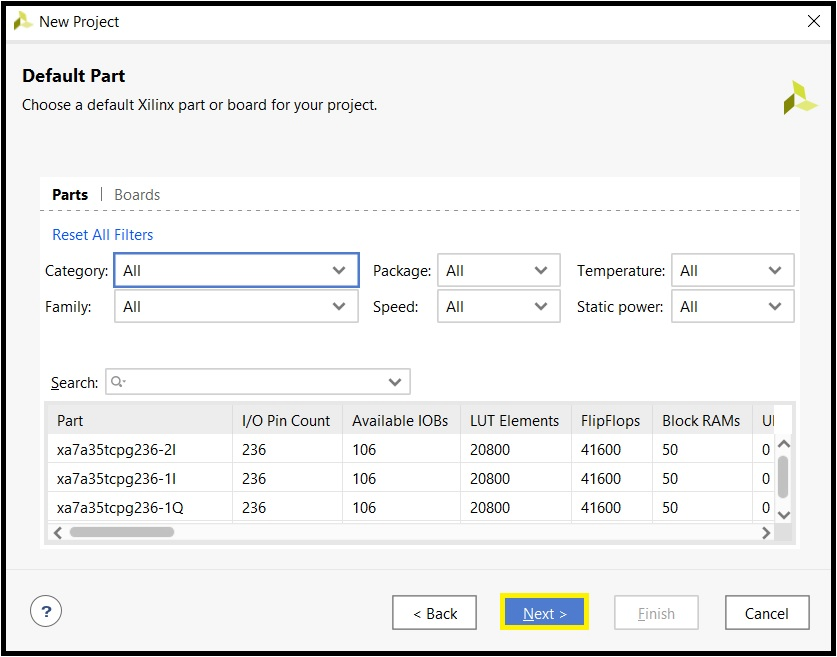
\includegraphics[width=0.7\linewidth]{images/vivado01f.png}
  \end{center}
\end{minipage}

\begin{minipage}{\linewidth}
  Step 1g: Click on "Finish": \\
  \begin{center}
    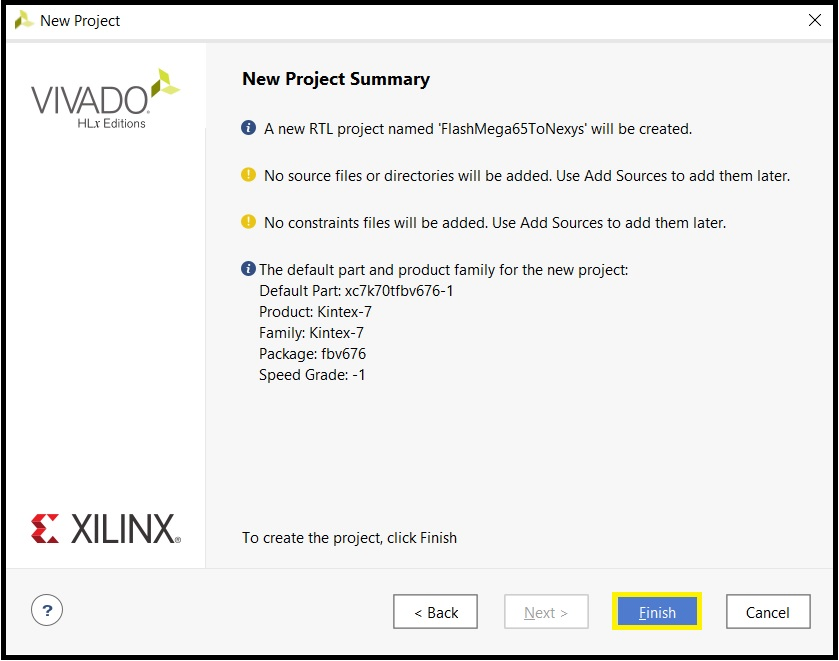
\includegraphics[width=0.8\linewidth]{images/vivado01g.png}
  \end{center}
\end{minipage}

\vspace{5mm}

\begin{minipage}{\linewidth}
  Step 2: In the left column, select "Open Hardware Manager"
  at the very bottom.
  \\
  \begin{center}
    \includegraphics[width=0.8\linewidth]{images/vivado02.png}
  \end{center}
\end{minipage}


\begin{minipage}{\linewidth}
  Step 3: Connect to the FPGA: \\
  Under "Open Hardware Manager", choose "Open Target", then "Auto Connect".
  \\
  \begin{center}
    \includegraphics[width=0.8\linewidth]{images/vivado03.png}
  \end{center}
\end{minipage}

\vspace{5mm}

\begin{minipage}{\linewidth}
  Step 4: Wait a moment, "Connecting to server..."  should
  automatically close without dropping an error to the console.
  \\
  \begin{center}
    \includegraphics[width=0.8\linewidth]{images/vivado04.png}
  \end{center}
\end{minipage}


\begin{minipage}{\linewidth}
  Step 5: Under "Open Hardware Manager", choose "Add Configuration
  Memory Device", then:
  \begin{itemize}
    \item \underline{For MEGA65R3/R3A/R4}: "xc7a200t\_0"
    \item \underline{For Nexys4 and MEGA65R2}: "xc7a100t\_0".
  \end{itemize}

  \begin{center}
    \includegraphics[width=0.7\linewidth]{images/vivado05.png}
  \end{center}
\end{minipage}

\vspace{5mm}

\begin{minipage}{\linewidth}
  Step 6a: Select Memory Part: \\
  \\
  In the newly opened dialogue:
  \begin{itemize}
    \item \underline{For MEGA65R2/R3}: type "S25fl256s"
    (without quotes), then select "s25fl256sxxxxxxx0-spi-x1\_x2\_x4"
    (the upper one) and click "OK".
    \item \underline{For MEGA65R3A/R4}: Vivado cannot flash the larger flash part on these boards. Use the flash menu on the MEGA65.
    \item \underline{For Nexys4}: type "S25fl128s"
    (without quotes), then select "s25fl128sxxxxxxx0-spi-x1\_x2\_x4"
    (the upper one) and click "OK".
  \end{itemize}

  \begin{center}
    \includegraphics[width=0.7\linewidth]{images/vivado06.png}
  \end{center}
\end{minipage}

\begin{minipage}{\linewidth}
  Step 6b: Click on "OK" to confirm you want to program the configuration memory device now.
  \begin{center}
    \includegraphics[width=0.85\linewidth]{images/vivado06b.png}
  \end{center}
\end{minipage}

\begin{minipage}{\linewidth}
  Step 6c: If you do not see such a popup, or wish to reprogram the QSPI on a future occasion, in "Hardware" window, right click on the memory configuration and select "Program Configuration Memory Device":
  \begin{center}
    \includegraphics[width=0.85\linewidth]{images/vivado06c.png}
  \end{center}
\end{minipage}

\begin{minipage}{\linewidth}
  Step 7: Set programming options: \\
  In the next dialogue, set the "Configuration file" to the path of your ".mcs" bitstream file. You can also optionally set the "PRM file" field to the path of your ".prm" file. Leave all other parameters
  as they are (see screenshot below).
  \\
  \begin{center}
    \includegraphics[width=0.85\linewidth]{images/vivado07.png}
  \end{center}
\end{minipage}

\vspace{1mm}

\begin{minipage}{\linewidth}
  Step 8: Patiently wait for the programming to finish.
  This can take several minutes as the Vivado software erases
  and then reprograms the flash memory that is used to
  initialise the FPGA on power-up.
  \\
  \begin{center}
    \includegraphics[width=0.85\linewidth]{images/vivado08.png}
  \end{center}
\end{minipage}


\begin{minipage}{\linewidth}
Step 9: If your screen looks like the screenshot below,
your new bitstream has been successfully flashed into Slot0 of your QSPI flash memory!
  \\
  \begin{center}
    \includegraphics[width=0.8\linewidth]{images/vivado09.png}
  \end{center}
\end{minipage}

\vspace{5mm}

\begin{minipage}{\linewidth}
Step 10: If you want to reflash the FPGA, you might find the
"Add Configuration Memory Device" option in step 5 greyed out.
Instead, select "s25fl256sxxxxxxx0-spi-x1\_x2\_x4"  in the "Hardware"
window, press right mouse button and select "Program Configuration
Memory Device" to flash.
  \\
  \begin{center}
    \includegraphics[width=0.8\linewidth]{images/vivado09.png}
  \end{center}
\end{minipage}


\section{Flashing the CPLD in the MEGA65's Keyboard with Lattice Diamond}


If you choose to proceed, you will need a TE0790-03 JTAG programming
module and a functioning installation of Lattice Diamond Programmer software.
This can be done on either Windows or Linux, but in both cases you will
need to install any necessary USB drivers. It is also necessary to have
dip-switches 1 and 3 in the ON position and dip-switches 2 and 4 in the
OFF position on the TE-0790. With your MEGA65 disconnected from the power,
the TE-0790 must be installed on the JB1 connector, which is located
between the floppy data cable and the audio jack.
The gold-plated hole of the TE-0790 must line up with the screw hole below.
The mini-USB cable will then connect on the side towards the 3.5" floppy drive.
The following image shows the correct position: The TE0790 is surrounded
by the yellow box, and the dip-switches by the red box. Dip-switch 1 is
the one nearest the floppy data cable.


\includegraphics[width=\linewidth]{images/jtag_detail_05.jpg}


On the PCB of a R2/R3/R3A/R4 MEGA65 mainboard, dip switch 1 (the one nearest to the user
sitting in front of the machine) must be in the ON position. The other
switches must be OFF. The keyboard will go into ``ambulance mode''
(blue flashing lights) when set correctly.

Connect your non-8-bit computer to the FPGA programming device using a
mini-USB cable. Switch the MEGA65 computer ON. Open the Diamond Programmer
which can be downloaded from the Internet.

\begin{minipage}{\linewidth}
Step 1: Open DIAMOND PROGRAMMER: \\
Select "Create a new project from a JTAG scan". If entry
under "Cable:" is empty, click "Detect Cable".
\\
  \begin{center}
  \includegraphics{images/diamond01.png}
  \end{center}
\end{minipage}

\vspace{5mm}

\begin{minipage}{\linewidth}
Step 2: Create a new project: \\
If dialog "Programmer: Multiple Cables Detected" appears,
select the first entry ("Location 0000") and click "OK".
  \begin{center}
  \includegraphics[width=0.7\linewidth]{images/diamond02.png}
  \end{center}
\end{minipage}


\begin{minipage}{\linewidth}
Step 3: Select cable: \\
You have now created a new project which should display
"MachXO2" under "Device Family" and "LCMXO2-1200HC" under "Device"
  \begin{center}
  \includegraphics[width=0.6\linewidth]{images/diamond03.png}
  \end{center}
\end{minipage}

\vspace{5mm}

\begin{minipage}{\linewidth}
Step 4: New Diamond Programmer project: \\
Choose "File" then "Open File" to load the Diamond Pprogrammer
project with the MEGA65 keyboard firmware update.
  \begin{center}
  \includegraphics[width=0.8\linewidth]{images/diamond04.png}
  \end{center}
\end{minipage}


\begin{minipage}{\linewidth}
Step 5: Open project: \\
Navigate into the folder with the extracted MEGA65 keyboard
firmware files you have received and select the file ending with ".xcf".
  \begin{center}
  \includegraphics[width=0.8\linewidth]{images/diamond05.png}
  \end{center}
\end{minipage}

\vspace{5mm}

\begin{minipage}{\linewidth}
Step 6: Select project file: \\
Click the three dots under "File Name" to set the correct
path and find the file ending with ".jed".
  \begin{center}
  \includegraphics[width=0.8\linewidth]{images/diamond06.png}
  \end{center}
\end{minipage}


\begin{minipage}{\linewidth}
Step 7: Choose correct path of .jed file: \\
Select the file ending with ".jed" and click "OK".
  \begin{center}
  \includegraphics[width=0.8\linewidth]{images/diamond07.png}
  \end{center}
\end{minipage}

\vspace{5mm}

\begin{minipage}{\linewidth}
  Step 8: Select .jed file: \\
Click on the icon with the green arrow facing down "PROGRAM",
which looks similar to the Diamond Programmer program icon.
  \begin{center}
  \includegraphics[width=0.8\linewidth]{images/diamond08.png}
  \end{center}
\end{minipage}


\begin{minipage}{\linewidth}
Step 9: Select cable: \\
After a moment the Output window should display
"INFO - Operation: successful." and the "Status" cell should
go green (does not always happen).
  \begin{center}
  \includegraphics[width=0.8\linewidth]{images/diamond09.png}
  \end{center}
\end{minipage}

\vspace{5mm}

\begin{minipage}{\linewidth}
Step 10: Operation successful: \\
You have now successfully flashed the MEGA65 keyboard.
If you wish you can now save the project for later use.
  \begin{center}
  \includegraphics[width=0.8\linewidth]{images/diamond10.png}
  \end{center}
\end{minipage}


\section{Flashing the MAX10 FPGA on the MEGA65's Mainboard with INTEL QUARTUS}

If you choose to proceed, you will need a TEI0004 - Arrow USB Programmer2 module with TEI0004 driver installed
and a functioning installation of Quartus Prime Programmer Lite Edition.  This can be done on either Windows
or Linux, but in both cases you will need to install any necessary USB drivers.
With your MEGA65 disconnected from the power, the TEI0004 must be installed on the J17 connector,
which is located between the floppy data cable and the ARTIX 7 FPGA on the Mainboard.
The micro-USB port of the TEI0004 must face in the opposite direction of the HDMI and LAN sockets, towards
the trap door.
The following image shows the correct position.

On the PCB R2/R3/R3A/R4 MEGA65 mainboard, all dip switches must be in the OFF position. The main FPGA of the MEGA65 must not contain
a valid bitstream. The easiest way to do this is if you have a TE0790 JTAG adapter: you can then use the m65 tool from a connected computer to begin sending a bitstream via JTAG, and then using control-C to abort the m65 tool before it can finish loading the bitstream.

\includegraphics[width=\linewidth]{images/jtag_detail_max10.png}

Connect your non-8-bit computer to the FPGA programming device using a micro-USB cable.
Open Quartus Prime Programmer Lite Edition, which can be downloaded from the Internet.

\begin{minipage}{\linewidth}
Step 1: Open Quartus Prime Programmer Lite Edition: \\
Click the "Hardware Setup" button in the top left corner of
the Quartus Prime Programmer window.
  \begin{center}
  \includegraphics{images/max10_01.png}
  \end{center}
\end{minipage}

\vspace{5mm}

\begin{minipage}{\linewidth}
Step 2: Enter Hardware Setup: \\
In the newly appeared window under "Currently selected
hardware" choose "Arrow-USB-Blaster".
If "Arrow-USB-Blaster" does not appear, verify cable and
drivers being correctly installed.
  \begin{center}
  \includegraphics[width=0.8\linewidth]{images/max10_02.png}
  \end{center}
\end{minipage}


\begin{minipage}{\linewidth}
Step 3: Select Arrow USB-Blaster: \\
Click the "Add File" button from the left row and choose the
latest ".pof" file. Then click "Open".
  \begin{center}
  \includegraphics[width=0.8\linewidth]{images/max10_03.png}
  \end{center}
\end{minipage}


\begin{minipage}{\linewidth}
Step 4: Select Programming File: \\
Tick at least the three boxes under "Program/Configure".
Also enabling all boxes under "Verify" and "Blank-Check"
will make the process more reliable.
  \begin{center}
  \includegraphics[width=0.7\linewidth]{images/max10_04.png}
  \end{center}
\end{minipage}

\vspace{5mm}

\begin{minipage}{\linewidth}
Step 5: Select Program/Configure Options:
  \begin{center}
  \includegraphics[width=0.7\linewidth]{images/max10_05.png}
  \end{center}
\end{minipage}

While keeping the Reset-Button pressed, switch the MEGA65 computer ON.
The keyboard will go into ``ambulance mode'' (blue flashing lights).
If it does not, the main FPGA is not empty - restart the whole process.

Now click on "Start" in the left row of buttons. The progress bar in
the top right corner should quickly go to 100 percent and turn green.
You have now successfully updated your MAX10 FPGA.

If you receive an error message instead, make sure the main FPGA
bitstream has been erased and that you did not release the reset-button on
the MEGA65 beforehand. Switch off the MEGA65 and restart this step.

\begin{minipage}{\linewidth}
Step 6: Programming successful:
  \begin{center}
  \includegraphics[width=0.8\linewidth]{images/max10_06.png}
  \end{center}
\end{minipage}

